
% Options for packages loaded elsewhere
\PassOptionsToPackage{unicode}{hyperref}
\PassOptionsToPackage{hyphens}{url}
\PassOptionsToPackage{dvipsnames,svgnames,x11names}{xcolor}
\documentclass{article}
\usepackage{xcolor}
\usepackage{amsmath,amssymb}
\setcounter{secnumdepth}{3}
\usepackage{iftex}
\usepackage{graphicx}
\makeatletter
\newsavebox\pandoc@box
\newcommand*\pandocbounded[1]{% scales image to fit in text height/width
  \sbox\pandoc@box{#1}%
  \Gscale@div\@tempa{\textheight}{\dimexpr\ht\pandoc@box+\dp\pandoc@box\relax}%
  \Gscale@div\@tempb{\linewidth}{\wd\pandoc@box}%
  \ifdim\@tempb\p@<\@tempa\p@\let\@tempa\@tempb\fi% select the smaller of both
  \ifdim\@tempa\p@<\p@\scalebox{\@tempa}{\usebox\pandoc@box}%
  \else\usebox{\pandoc@box}%
  \fi%
}
% Set default figure placement to htbp
\def\fps@figure{htbp}
\makeatother
\ifLuaTeX
\usepackage[bidi=basic,shorthands=off]{babel}
\else
\usepackage[bidi=default,shorthands=off]{babel}
\fi
\ifLuaTeX
  \usepackage{selnolig} % disable illegal ligatures
\fi
\setlength{\emergencystretch}{3em} % prevent overfull lines
\providecommand{\tightlist}{%
  \setlength{\itemsep}{0pt}\setlength{\parskip}{0pt}}
\usepackage[]{natbib}
\bibliographystyle{iclr2027_conference}
\usepackage{iclr2027_conference,times}
\renewcommand{\arraystretch}{1.35}
\ifdefined\extrarowheight\setlength{\extrarowheight}{3pt}\fi
% Table rows here carry phrases, not single words, and pandoc's longtables set
% them solid. Both knobs are needed: \arraystretch scales the row strut,
% \extrarowheight lifts the text off the rule above it.
\renewcommand{\arraystretch}{1.35}
% pandoc loads these only when the main text has a table; a paper whose tables all sit
% in the appendix still needs them, and \extrarowheight needs array either way
\usepackage{longtable,booktabs,array,calc}
% pandoc numbers a caption-less table against a counter named none, defined with the rest
\makeatletter\@ifundefined{c@none}{\newcounter{none}}{}\makeatother
\setlength{\extrarowheight}{3pt}
\usepackage{bookmark}
\IfFileExists{xurl.sty}{\usepackage{xurl}}{} % add URL line breaks if available
\urlstyle{same}
\ifdefined\captionsetup\captionsetup{font=small}\fi
% Float placement, on every face. LaTeX's defaults reserve most of a page for
% text, so a tall figure is deferred past the section that introduces it. These
% let a float take more of the page it belongs on, and `!htbp` adds "here".
\renewcommand{\topfraction}{0.92}
\renewcommand{\bottomfraction}{0.85}
\renewcommand{\textfraction}{0.06}
\renewcommand{\floatpagefraction}{0.72}
\setcounter{topnumber}{3}
\setcounter{bottomnumber}{2}
\setcounter{totalnumber}{4}
\makeatletter
\renewcommand{\fps@figure}{!htbp}
\renewcommand{\fps@table}{!htbp}
% A float still waiting when a numbered section begins is flushed first, so a
% figure stays inside the section that cites it. placeins would do this, but
% it is not in a BasicTeX installation. \@deferlist holds exactly the pending
% floats, so the page only breaks when one is actually waiting.
\newcommand{\iclr@floatbarrier}{\par\vspace{\z@}%
  \ifx\@deferlist\@empty\else\clearpage\fi}
\let\iclr@section\section
\renewcommand{\section}{\iclr@floatbarrier\iclr@section}
\makeatother
% fallback for those not using the hyperref driver hyperxmp:
\makeatletter
\@ifundefined{xmpquote}{\newcommand{\xmpquote}[1]{#1}}{}
\makeatother
\hypersetup{
  pdftitle={Spoken-Digit Recognition Without Training: Geometry{,} Coupling{,} and Drive Effects in Oscillator Networks},
  pdflang={en-GB},
  pdfkeywords={\xmpquote{coupled oscillators}, \xmpquote{reservoir
computing}, \xmpquote{speech recognition}, \xmpquote{Kuramoto
model}, \xmpquote{Stuart-Landau}, \xmpquote{lattice geometry}},
  colorlinks=true,
  linkcolor={RoyalBlue},
  filecolor={Maroon},
  citecolor={RoyalBlue},
  urlcolor={RoyalBlue},
  pdfcreator={LaTeX via pandoc}}
\hypersetup{pdfauthor={}}
\hypersetup{pdfcreator={}, pdfproducer={}}
\ifdefined\pdftrailerid\pdftrailerid{}\fi
\ifdefined\pdfsuppressptexinfo\pdfsuppressptexinfo=-1\fi
\ifdefined\pdfinfoomitdate\pdfinfoomitdate=1\fi
\ifdefined\pdfvariable\pdfvariable suppressoptionalinfo 1023\relax\fi
\ifdefined\pdfgentounicode\input{glyphtounicode}\pdfgentounicode=1\fi
\title{Spoken-Digit Recognition Without Training: Geometry, Coupling,
and Drive Effects in Oscillator Networks}

\author{Eric Kryski \\
Independent researcher \\
\texttt{hello@erickryski.com}}

\begin{document}
\maketitle
\def\iclrface{submission}\def\iclrpreprint{preprint}
\ifx\iclrface\iclrpreprint\lhead{}\fi
\begin{abstract}
Coupled-oscillator networks are gaining interest as a machine-learning
substrate, on the premise that oscillator physics turns signals into
useful structure. Yet the ablations that would isolate what the
oscillator dynamics contribute are rarely run. We run them for untrained
coupled oscillator networks, using spoken-digit classification on
AudioMNIST as the measure. A small untrained network is read by a
closed-form linear readout and compared with five trained conventional
networks (GRU, TCN, CNN, transformer and S4D) matched in parameters and
with three controls: the same network with its coupling removed, a
non-oscillating bank of leaky integrators with the same states and
parameters, and the same readout fitted directly to the network's input.
Every experimental arm's state is summarized by the same time-pooled
statistics and spoken digits classified using the same number of
features, so that readout capacity cannot mask dynamics. The ablations,
eight experiments of 6,353 runs in all, vary six coupling functions,
eight lattice geometries, and the natural frequencies, input pathway,
input gain, readout width and training set size, on digit recognition
and on a temporal order task that order-blind readouts cannot solve. The
design separates three explanations for an untrained network's accuracy:
its input representation, the width of its readout, and the oscillator
dynamics and structure themselves. Our ablation study results give
future studies of trained oscillator networks an untrained baseline to
compare against for speech recognition tasks, and insight into which
factors contribute to an oscillator network's effectiveness on
time-series tasks.
\end{abstract}

\section{Introduction}\label{sec-1}

Every sense we have transduces a physical signal, and the oscillation
and synchronization recorded in neural populations as they track speech
\citep{assaneo2020, doelling2023, pittman-polletta2021, dogonasheva2026}
are consistent with neurons acting, in part, as coupled oscillators. We
do not test that conjecture here. It motivates a narrower question:
where are the useful boundaries of oscillatory neural networks, and what
do their dynamics contribute?

A recent survey of oscillator networks in machine learning
\citep{kryski2026} found the ablations that would answer that question
largely missing: the coupling term had been removed as a single variable
only three times, coupling functions had been compared only within the
Kuramoto family \citep{nunley2026}; one graph network has since set
Stuart--Landau against Kuramoto, without fixing the amplitude
\citep{zhang2026}. No study varied the lattice geometry or its
boundaries as a single variable at a matched budget, and none contrasted
different audio input structures under controls. We address those gaps
on one task, spoken-digit recognition, where automatic speech
recognition began \citep{davis1952} and a standard benchmark for
oscillator reservoirs built in hardware
\citep{torrejon2017, shougat2023}. An untrained coupled oscillator
network, read by a linear readout, is tested under six coupling
functions and eight lattice geometries, among them a coil and a cochlea,
and compared with the readout applied to its input alone, the same
network uncoupled, leaky-integrator banks of the same size and five
trained networks of the same parameter count, on AudioMNIST
\citep{becker2024} with held-out speakers and added noise. Untrained
networks of coupled oscillators have recognized spoken digits before, in
simulation and on TI-46 with the same speakers in training and test
\citep{opala2019, coulombe2017}. To our knowledge none have been tested
on held-out speakers with added noise against their input alone and
their own uncoupled form. Additionally, we found no AudioMNIST result
that combines held-out speakers with added noise. The two studies we
found that add noise on AudioMNIST share speakers between training and
test \citep{beoletto2026, young2026}.

\section{Background}\label{sec-2}

Coupled oscillators synchronize, form clusters, lock to a drive or split
into coherent and incoherent domains, depending on how they are coupled
and arranged
\citep{pikovsky2001, strogatz2000, kuramoto2002, abrams2004}. Machine
learning has used them two ways. Untrained, as reservoirs read by a
trained linear readout \citep{jaeger2001, maass2002, tanaka2019}: a
spintronic oscillator recognized spoken digits in hardware
\citep{torrejon2017}, though much of that accuracy came from its
cochlear front end \citep{abreu-araujo2020}, whose authors therefore
report a reservoir's gain over its front end alone and test it on
held-out speakers in noise on another corpus. On AudioMNIST, a simulated
network of 128 coupled protonic nickelate devices, a neuromorphic
element that does not oscillate, read above the same network uncoupled
and above a readout of the unprocessed input \citep{zhou2026}, which
inspired one of the controls used in our study. Trained oscillatory
neural networks (ONNs), structured as layers whose coupling or
frequencies are learned, have been applied to various tasks: Neural Wave
Machines, an oscillator lattice, on sequence classification and
forecasting simple physical systems \citep{keller2023}, AKOrN on
unsupervised object discovery, adversarial robustness, uncertainty
calibration and Sudoku \citep{miyato2025}, WONN on image recognition,
Sudoku and maze solving \citep{dai2026}, FSN on character-level language
modelling \citep{nunley2026}, Un-0 on image generation
\citep{unconv-ai2026} and coupled oscillatory recurrent networks, coRNN
\citep{rusch2021}, one of which reached 89\% on AudioMNIST from the raw
waveform with a random, not speaker-disjoint, split
\citep{chandravadia2026}. Most adopt one coupling function and one
arrangement, and the survey found that few share a benchmark, AKOrN and
WONN on Sudoku among them, and fewer share a protocol
\citep{kryski2026}. Here one task is held fixed and the coupling
function, the geometry and the input are varied across it, on untrained
networks, so that each can be compared with controls in future training
experimentation.

\section{Methods}\label{sec-3}

\subsection{Design}\label{sec-3-1}

This study asks whether an untrained coupled oscillator network carries
information for recognizing spoken digits beyond its input alone, beyond
a non-oscillating memory of the same size and beyond the same
oscillators uncoupled; how trained networks of the same parameter count
compare; whether the coupling function, lattice geometry, natural
frequencies, restoring strength, coupling ceiling, input pathway and
input gain change the answer; how the answer changes with the readout's
width and the training data; and whether an untrained network can
\emph{remember} the order of events. It ran as eight experiments with
6,353 single-control ablation experimentation runs in total. Every run
is one arm at one noise level, input gain and seed, and every condition
is run at three seeds. The code and every run's record, with a README
for each experiment and a summary of every result, are in the
supplementary material, and \hyperref[sec-A]{Appendix A} defines every
term.

Every oscillator network is 4 channels of a 16 \ensuremath{\times} 16
lattice, 1,024 oscillators, and each oscillator's phase evolves as
\ensuremath{\dot{\theta}_{i}} = \ensuremath{\omega_{i}} +
coupling\ensuremath{_{i}} + g\ensuremath{\cdot}u\ensuremath{_{i}}
\ensuremath{-} \ensuremath{\lambda} sin \ensuremath{\theta_{i}}: its
natural frequency, the coupling from the other oscillators of its
channel through a random kernel whose spectrum is capped at the
\emph{coupling ceiling}, the input at gain g, and a restoring pull of
strength \ensuremath{\lambda}. Row r of every channel is driven by mel
band r. The six coupling functions (Kuramoto, Kuramoto--Sakaguchi,
second harmonic, Winfree, and Stuart--Landau with and without its
amplitude) differ only in the coupling term, and a lattice geometry
changes only which oscillators are neighbours (see
\hyperref[sec-B]{Appendices B} and \hyperref[sec-C]{C}). The reference
configuration is Kuramoto coupling on the torus with random natural
frequencies, restoring strength 0.3 and coupling ceiling 1.

The arms compared with it are the \textbf{spectrogram-only baseline},
the readout applied directly to the input; the \textbf{uncoupled
oscillator network}, the same network with its coupling kernels set to
zero; two untrained \textbf{leaky-integrator banks}, one matched to the
network's 1,024 states and 2,048 parameters and one to its 2,048 exposed
signals; and five \textbf{trained baselines} (GRU, a dilated residual
TCN, CNN, transformer and S4D) of 1,840 to 2,109 parameters, trained end
to end (AdamW, 30 epochs) through a learned linear layer on the same
statistics the readout reads, standardized. The four untrained dynamical
arms are the reservoirs.

\subsection{Task, data and noise}\label{sec-3-2}

We perform single-digit audio classification over AudioMNIST
\citep{becker2024}, which holds 30,000 recordings of digits 0 through 9
by 60 speakers. Every result keeps speakers apart to avoid a model
overfitting to a particular speaker's vocal spectrogram. Under Protocol
A the arms train on speakers 1 to 48 and test on all 6,000 recordings of
speakers 49 to 60, an 80/20 split by speaker, with training sets of
2,048 clips (8,192 and 24,000 in the training-size comparison). Under
Protocol B they follow Becker et al.'s five speaker folds (60/20/20).
Because the clean task nearly saturates, white noise is added to every
clip at signal-to-noise ratios of 0 dB (as loud as the speech) and
\ensuremath{-}5 dB (5 dB louder), the levels at which \citet{young2026}
trained hybrid real and complex-valued convolutional networks on
AudioMNIST, though they did so on a random audio sample split so were
not speaker disjoint. We also report clean audio for reference.
Additionally, we performed an order task on five different digit pairs
where two digits of a pair are spoken one after the other and the arm
must say which came first. Statistics of an input read over the whole
span cannot tell the orders apart, so the spectrogram-only baseline
reads chance, 50\%. Every arm hears the same fixed front end, a 16-band
log-mel spectrogram at 62.5 frames per second, without training on this
task besides the single-digit training methodology.

\subsection{Readout}\label{sec-3-3}

Every arm is read the same way (\hyperref[sec-D-1]{Appendix D.1} draws
the readout for each kind of arm). Each of its signals (a band energy,
the sine or cosine of an oscillator's phase, a leaky integrator's state
or a trained baseline's hidden unit) is summarized by its mean, standard
deviation and mean absolute change over each of four equal windows of
frames 16 to 61, after a 16-frame warm-up (frames 16 to 147 as one
window for the order task). So that readout capacity cannot obscure
dynamics, every arm is read at the same width, 192 standardized
features. That is exactly the spectrogram-only baseline's own number of
features (16 mel bands by 3 statistics by 4 windows), so the input is
read without compression, and it is the native width of four of the five
trained baselines. Arms with more features, the reservoirs (12,288 to
24,576) and the GRU (216), are projected down to 192 by a random
Gaussian matrix \citep{johnson1984}. Arms with fewer features, the
baseline and the trained baselines on the order task (48 to 54), are
read as they are. Widths of 1,024 and 4,096 show what the projection
costs in terms of classification quality. The features are classified by
one linear layer fitted by ridge regression in closed form, the
reservoir-computing standard \citep{jaeger2001, lukosevicius2012} and
the weakest reader that can be fitted identically for every arm. The
projection matrix is drawn once, from a fixed random seed, and the same
matrix serves every run of the same native width whatever its run seed,
so the spread over seeds leaves out the projection's own randomness; the
controls experiment's reservoirs are also read through a matrix drawn
from each run's seed, which includes it. The spectrogram-only baseline
is read over the whole clip, its primary form, and from frame 16, the
frames every other arm is read over.

\subsection{Input pathways and gain}\label{sec-3-4}

The audio drives a reservoir in one of two ways: the
\textbf{spectrogram} pathway adds each band's energy to the rotation
rate of its row's oscillators, and the \textbf{quadrature} pathway adds
a phase-referenced push g\ensuremath{\cdot}A\ensuremath{_{r}}
sin(\ensuremath{\varphi_{r}} \ensuremath{-} \ensuremath{\theta_{i}}),
the injection form of \citet{adler1946}, so an oscillator can lock to
its band's own cycle. Only the coupled networks run on the quadrature
pathway, beside its own spectrogram-only baseline, which reads the
quadrature front end directly: a leaky integrator has no phase for the
push to act on, the trained baselines take the input as features rather
than as a drive, and the uncoupled network was left out because the
question is whether coupled oscillators can use a phase-referenced drive
at all. Input gain scales the input into a reservoir; it is run at gains
of 1 and 2 throughout and swept from 0.25 to 12 for the reference
configuration of each coupling function, below the integrator's bound
\citep{hairer1993}. The spectrogram-only baseline and the trained
baselines do not have gain applied because the readout's standardization
removes any fixed scale from the directly read spectrogram input, and
the trained models learn their own.

\subsection{Reporting}\label{sec-3-5}

Every task accuracy result reported is the mean over replicates (three
seeds; five folds under Protocol B) \ensuremath{\pm} the sample standard
deviation, and every comparison between two arms is paired on the same
test clips, condition and seed, reported as the mean difference
\ensuremath{\pm} its standard deviation over seeds and a 95\% interval
from 2,000 paired bootstrap resamples of the test clips. Every
comparison is reported at the primary cell, the four-window read at
2,048 training clips and readout width 192, unless it says otherwise.

\section{Results}\label{sec-4}

\subsection{The network against its controls and the trained
baselines}\label{sec-4-1}

\hyperref[fig-c3-recognition-arms]{Figure 1} shows every arm at the
primary cell, and the supplementary material gives the tables. The
spectrogram-only baseline read 93.6\%, 78.0\% and 71.6\% on clean audio,
at 0 dB and at \ensuremath{-}5 dB, and the Kuramoto network at gain 1
read 91.1\%, 77.8\% and 70.7\%: within a point of its input with noise
(\ensuremath{-}0.23 {[}\ensuremath{-}0.99, +0.52{]} at 0 dB,
\ensuremath{-}0.88 {[}\ensuremath{-}1.66, \ensuremath{-}0.09{]} at
\ensuremath{-}5 dB) and 2.53 points below it on clean audio, but 7.5 to
15.9 points above the input read over the same frames, from frame 16. It
read 0.43 to 1.08 points above the uncoupled network, and about 4 points
above the state-matched leaky-integrator bank with noise but 2.35 points
below it on clean audio; gain 2 read lower than gain 1 for every control
reservoir. The Stuart--Landau network read 93.9\%, 80.3\% and 73.0\%
(gain 1), level with its input on clean audio (+0.28 points) and above
it in every noisy condition (\hyperref[sec-4-3]{Section 4.3}). With
noise every trained baseline read above the Kuramoto network, from
79.2\% (CNN) to 82.8\% (GRU) at 0 dB and 72.3\% (transformer) to 76.9\%
(GRU) at \ensuremath{-}5 dB, with the Stuart--Landau network in their
range; on clean audio they read 94.7\% to 97.0\%. On the speaker folds
of \citet{becker2024} (clean, 18,000 training clips), the baseline read
96.0 \ensuremath{\pm} 1.7\%, the network 91.9 \ensuremath{\pm} 3.1\%
(96.9 \ensuremath{\pm} 1.3\% at width 4,096) and the trained baselines
97.0\% to 98.4\%, against 95.8\% reported for AlexNet on spectrograms.

\begin{figure}
\centering
\pandocbounded{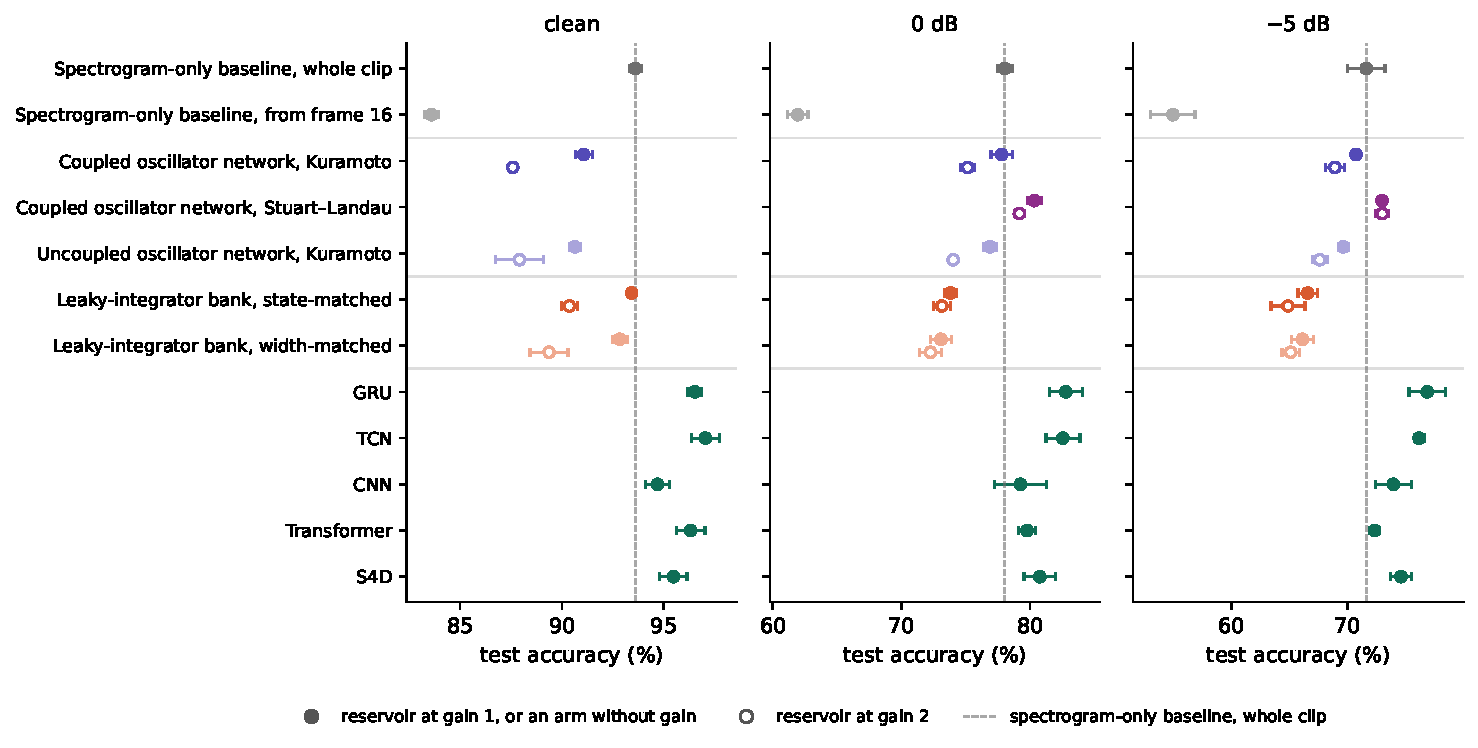
\includegraphics[keepaspectratio,alt={Recognition accuracy per arm and noise level at the primary cell (width 192, 2,048 training clips); mean  one standard deviation over three seeds. Reservoirs at gain 1 (filled) and 2 (open). The oscillator networks are the Kuramoto reference configuration and the same with Stuart--Landau coupling. Dashed line: the whole-clip spectrogram-only baseline.}]{resources/figures/c3-recognition-arms.pdf}}
\caption{Recognition accuracy per arm and noise level at the primary
cell (width 192, 2,048 training clips); mean \ensuremath{\pm} one
standard deviation over three seeds. Reservoirs at gain 1 (filled) and 2
(open). The oscillator networks are the Kuramoto reference configuration
and the same with Stuart--Landau coupling. Dashed line: the whole-clip
spectrogram-only baseline.}\label{fig-c3-recognition-arms}
\end{figure}

\subsection{Temporal order}\label{sec-4-2}

\hyperref[fig-c8-order-arms]{Figure 2} shows every arm on the two digit
ordered classification task, averaged over the five digit pairs; the
supplementary material gives the table. The spectrogram-only baseline
read 49.8\% to 50.6\% on the order task in every condition. The Kuramoto
network read 97.7\%, 96.2\% and 95.5\% at gain 1 (clean, 0 dB,
\ensuremath{-}5 dB), 45.4 to 47.9 points above it; uncoupled, it read
2.2 to 8.5 points lower at gain 1 and 10.4 to 18.7 points lower at gain
2. Both leaky-integrator banks read 98.7\% to 99.9\%, 2.2 to 7.5 points
above the network. The transformer and GRU read 99.0\% to 99.9\%, the
S4D 96.9\% to 99.1\% and the TCN 91.1\% to 99.9\%. The CNN read 92.2\%
on clean audio and chance with noise: its two convolutions see 9 frames
(144 ms), less than a digit, so with no memory beyond that window it can
tell the orders apart only where one digit meets the other, a cue the
noise masks.

\begin{figure}
\centering
\pandocbounded{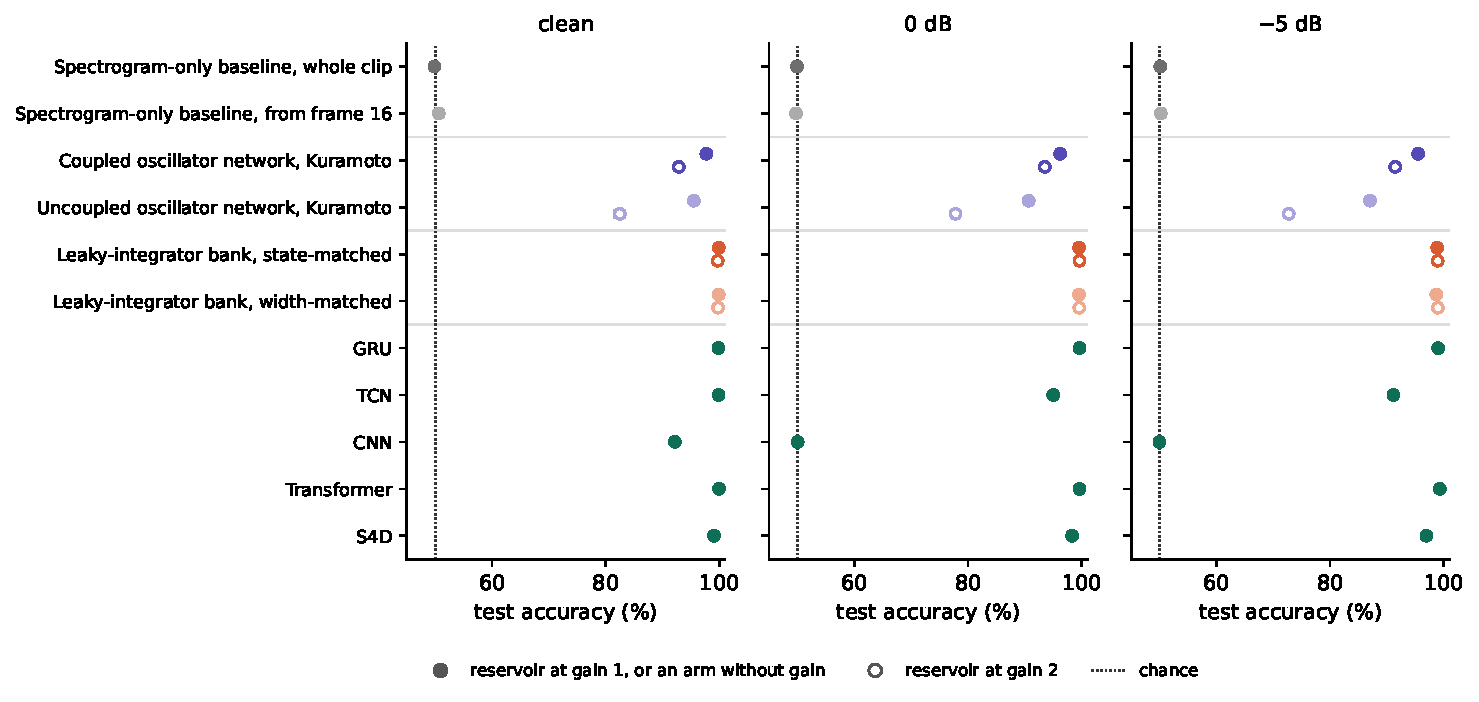
\includegraphics[keepaspectratio,alt={Temporal-order accuracy per arm and noise level, averaged over five digit pairs; mean  one standard deviation over three seeds, at most 0.8 points and hidden by the markers. Reservoirs at gain 1 (filled) and 2 (open), read at width 192; the baselines' 48 to 54 features are read as they are. Dotted line: chance.}]{resources/figures/c8-order-arms.pdf}}
\caption{Temporal-order accuracy per arm and noise level, averaged over
five digit pairs; mean \ensuremath{\pm} one standard deviation over
three seeds, at most 0.8 points and hidden by the markers. Reservoirs at
gain 1 (filled) and 2 (open), read at width 192; the baselines' 48 to 54
features are read as they are. Dotted line:
chance.}\label{fig-c8-order-arms}
\end{figure}

\subsection{Coupling function}\label{sec-4-3}

The design experiment crossed six coupling functions, six lattice
geometries, three kinds of natural frequencies, two restoring strengths
and two coupling ceilings (the Stuart--Landau functions on the torus
only), 312 configurations at 0 and \ensuremath{-}5 dB, gains 1 and 2 and
three seeds, each level paired with its reference over every
configuration matching it in the other factors
(\hyperref[fig-c4-coupling-functions]{Figure 3}). The
\textbf{Stuart--Landau} network, whose oscillators have a free
amplitude, read 2.1 to 3.8 points above its Kuramoto match, the largest
difference in the experiment, and at the reference configuration it read
above the whole-clip baseline in all four noisy conditions, by 1.14 to
2.31 points with every interval above zero; with its amplitude fixed it
read within 0.3 points of Kuramoto. The other phase coupling functions
differed from Kuramoto by at most 0.46 points.

\begin{figure}
\centering
\pandocbounded{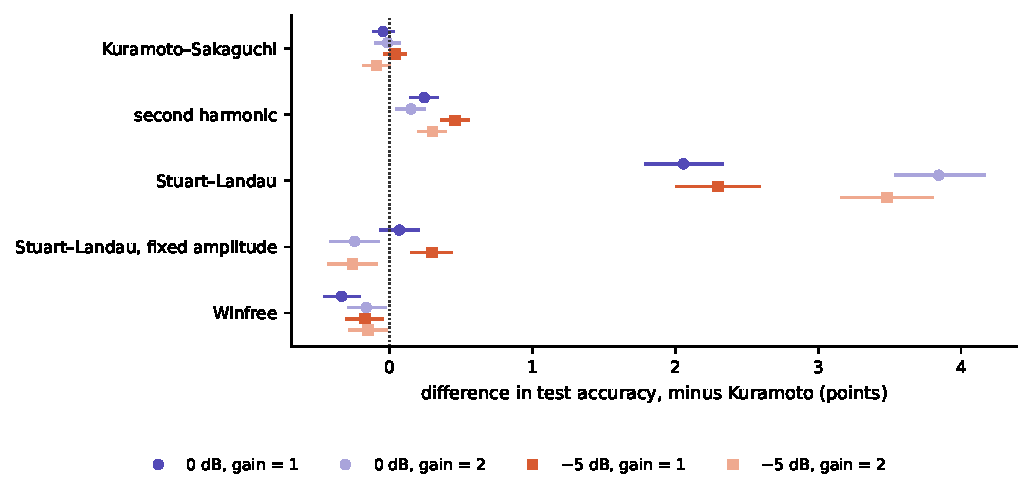
\includegraphics[keepaspectratio,alt={Each coupling function minus Kuramoto, per noise level and gain, paired over matching configurations: mean over three seeds (marker) and 95\% paired bootstrap interval (line). Dotted line: no difference.}]{resources/figures/c4-coupling-functions.pdf}}
\caption{Each coupling function minus Kuramoto, per noise level and
gain, paired over matching configurations: mean over three seeds
(marker) and 95\% paired bootstrap interval (line). Dotted line: no
difference.}\label{fig-c4-coupling-functions}
\end{figure}

\subsection{Lattice geometry and natural frequencies}\label{sec-4-4}

Every \textbf{lattice geometry} in the design experiment read within
0.65 points of the torus, the sphere and sheet lowest
(\hyperref[fig-c4-lattice-geometries]{Figure 4}). A \textbf{coil}, one
open line from base to apex with one octave per turn, read within 0.22
points of the torus; a \textbf{cochlea}, the coil with coupling three
times as strong from base to apex as back and growing with the coil's
curvature toward the apex, read 0.41 to 0.97 points below the torus.
Part of that gap is the cochlea's weaker coupling: capping its curvature
weights at the apex halves its average coupling, and a control at the
coil's average coupling read 0.28 to 0.71 points above the cochlea, yet
0.40 to 0.47 points below the coil at gain 1 and within 0.12 points of
it at gain 2.

\begin{figure}
\centering
\pandocbounded{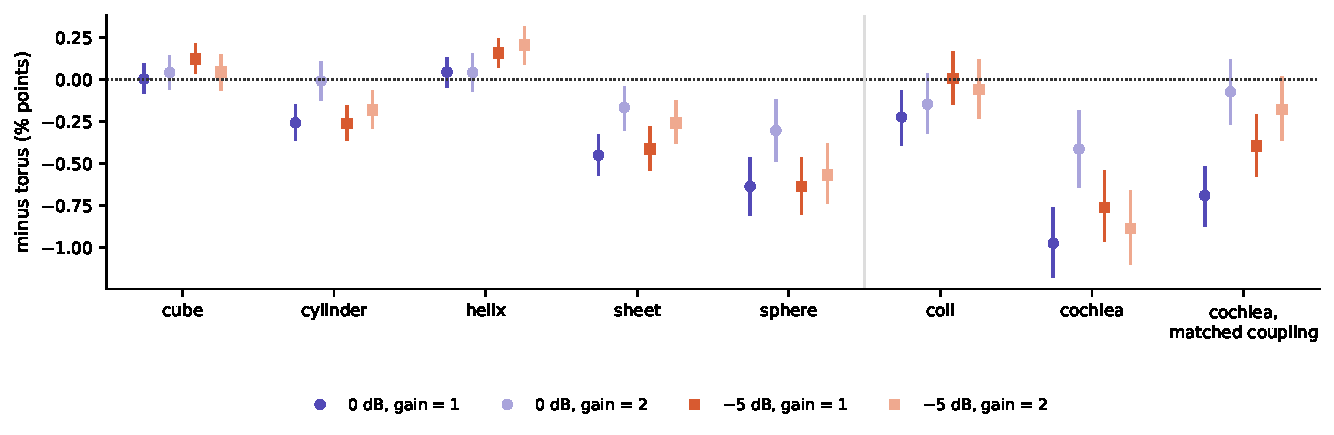
\includegraphics[keepaspectratio,alt={Each lattice geometry minus the torus, per noise level and gain: mean over three seeds (marker) and 95\% paired bootstrap interval (line). Left of the grey line, the design experiment, paired over matching configurations; right, the cochlea experiment, paired over its twelve. Dotted line: no difference.}]{resources/figures/c4-lattice-geometries.pdf}}
\caption{Each lattice geometry minus the torus, per noise level and
gain: mean over three seeds (marker) and 95\% paired bootstrap interval
(line). Left of the grey line, the design experiment, paired over
matching configurations; right, the cochlea experiment, paired over its
twelve. Dotted line: no difference.}\label{fig-c4-lattice-geometries}
\end{figure}

Each oscillator's \textbf{natural frequency} is its rate of rotation
when nothing acts on it. The reference draws each at random with mean 1
and standard deviation 0.1, unrelated to the band that drives it.
\textbf{Tonotopic} frequencies order the rates by band, as the cochlea
orders pitch by place: the rate rises a quarter octave per row, from
0.41 in the row of the lowest mel band to 5.5 in the highest, jittered
by 5\%. \textbf{Identical} frequencies set every rate to 1. Tonotopic
frequencies read 0.38 to 1.16 percentage points below random ones, and
identical ones within 0.1 (\hyperref[fig-c4-natural-frequencies]{Figure
5}).

\begin{figure}
\centering
\pandocbounded{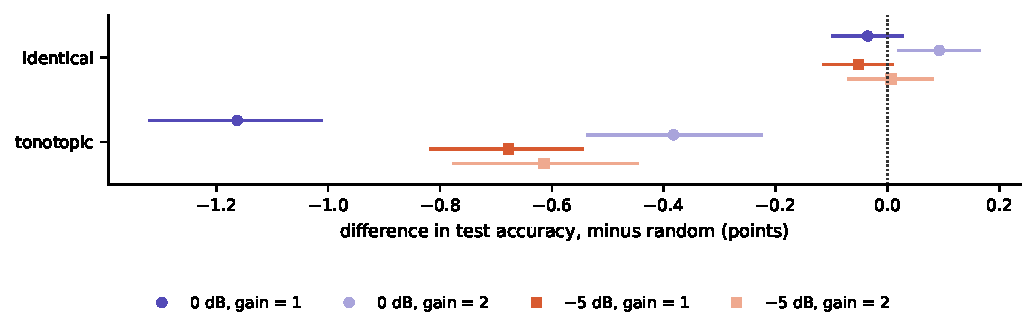
\includegraphics[keepaspectratio,alt={Identical and tonotopic natural frequencies minus random ones, paired and drawn as for the coupling functions. Dotted line: no difference.}]{resources/figures/c4-natural-frequencies.pdf}}
\caption{Identical and tonotopic natural frequencies minus random ones,
paired and drawn as for the coupling functions. Dotted line: no
difference.}\label{fig-c4-natural-frequencies}
\end{figure}

\subsection{Restoring strength, coupling ceiling and
gain}\label{sec-4-5}

A restoring strength (the pull toward phase 0) of 0.1 read 0.13 to 0.23
points below 0.3, and a coupling ceiling of 0.5 read 0.39 to 0.68 points
below 1. A sweep beyond these levels, for every coupling function at the
reference configuration, found restoring strengths of 0.5 to 1.0 moving
the phase-oscillator networks by \ensuremath{-}1.2 to +2.1 points and
lowering the Stuart--Landau network in every condition, by 0.4 to 2.8
points, and ceilings of 1.5 and 2 moving every coupling function by
\ensuremath{-}2.4 to +1.7 points. Gain separates the Stuart--Landau
network from the rest (\hyperref[fig-c6-restoring-ceiling-gain]{Figure
6}): from gain 1 to gain 8 it lost 4.3 points at 0 dB and 2.8 at
\ensuremath{-}5 dB, while every phase-oscillator network lost 15 to 19
points and the Stuart--Landau network with its amplitude fixed 25 to 28;
beyond gain 8 it also gave way, losing 8.4 points by gain 10 and 20.8 by
gain 12 at 0 dB. Below gain 1 the order reverses: at gains 0.25 and 0.5
the phase-oscillator networks and the fixed-amplitude network read 0.3
to 2.5 points above gain 1 and the Stuart--Landau network 0.7 to 1.7
points below it. At its better low gain every phase-oscillator network
read above its input at 0 dB, by 0.7 to 1.6 points, and the
second-harmonic network at \ensuremath{-}5 dB too, by 1.4, which brings
the best of them within 0.8 points of the Stuart--Landau network at gain
1 at 0 dB and level with it at \ensuremath{-}5 dB.

\begin{figure}
\centering
\pandocbounded{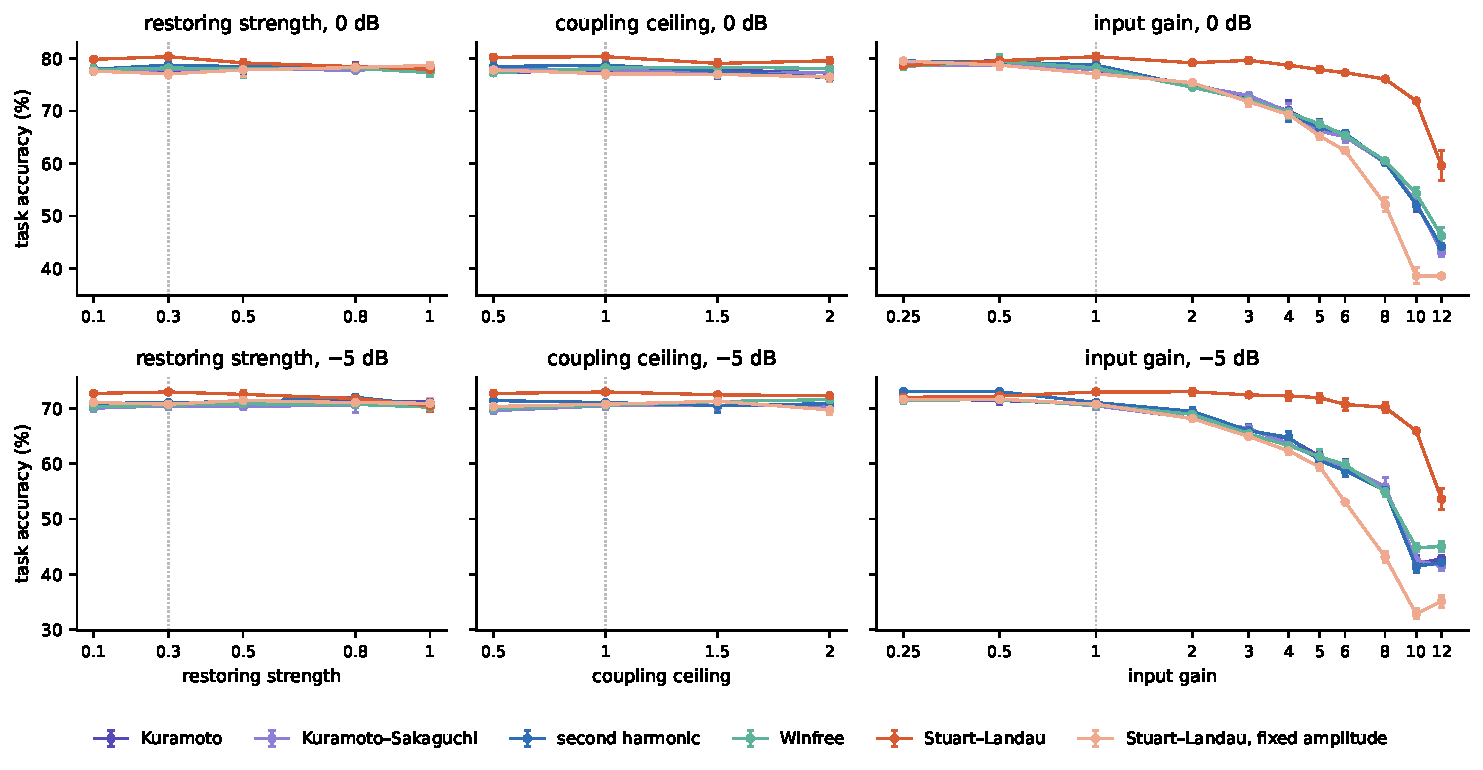
\includegraphics[keepaspectratio,alt={Accuracy of each coupling function at the reference configuration against restoring strength and coupling ceiling (gain 1) and against input gain, at 0 dB (top) and 5 dB (bottom), 2,048 training clips; mean  one standard deviation over three seeds. Dotted line: the reference setting.}]{resources/figures/c6-restoring-ceiling-gain.pdf}}
\caption{Accuracy of each coupling function at the reference
configuration against restoring strength and coupling ceiling (gain 1)
and against input gain, at 0 dB (top) and \ensuremath{-}5 dB (bottom),
2,048 training clips; mean \ensuremath{\pm} one standard deviation over
three seeds. Dotted line: the reference
setting.}\label{fig-c6-restoring-ceiling-gain}
\end{figure}

\subsection{Quadrature pathway}\label{sec-4-6}

The quadrature experiment ran a subset of the design's configurations on
the quadrature pathway: each of the four phase coupling functions
(Kuramoto, Kuramoto--Sakaguchi, second harmonic and Winfree) on the
torus, and Kuramoto on the helix as well, each with random and with
tonotopic natural frequencies, at the reference restoring strength and
coupling ceiling. That is ten networks, each at 0 and \ensuremath{-}5
dB, gains 1 and 2 and three seeds; the other four geometries and the two
Stuart--Landau functions were not run on this pathway. All ten read
11.7\% to 15.1\%, near the chance level of 10\% and 55.7 to 66.0 points
below the same networks on the spectrogram pathway, while the
spectrogram-only baseline read on the quadrature front end reached
36.1\% at 0 dB. Their oscillators did not lock to the drive: in no run
did more than 0.3\% of them lock to their band above a phase-locking
value of 0.5.

\subsection{Readout width and training data}\label{sec-4-7}

Widening the readout to 1,024 and 4,096 features raised nearly every arm
with more than 192 features to read, the Kuramoto network by up to 3.8
points at gain 1 (6.3 at gain 2) and the leaky-integrator banks by up to
6.2, and left the 192-wide arms unchanged
(\hyperref[fig-c9-readout-width]{Figure 7}; \hyperref[sec-D-1]{Appendix
D.1} shows the reader structure). From 2,048 to 24,000 training clips,
at width 192 and with noise, the spectrogram-only baseline gained 3.5 to
4.1 points, the Kuramoto network 2.0 and the trained baselines 7.1 to
12.4, since they learn through their networks as well as their readout.
At width 4,096 the Kuramoto network read above the whole-clip
spectrogram-only baseline at every training size, and with 2,048 clips
at 0 dB above the S4D, CNN and transformer (81.4\% against 79.2\% to
80.8\%), though through a readout with more weights than theirs; with
8,192 or 24,000 clips every trained baseline read above every reservoir
at every width with noise. Read through the seeded projection instead of
the fixed one, the controls experiment's reservoirs moved by
\ensuremath{-}1.29 to +1.22 points (median \ensuremath{-}0.06), and
every paired comparison between the controls arms kept its sign.

\begin{figure}
\centering
\pandocbounded{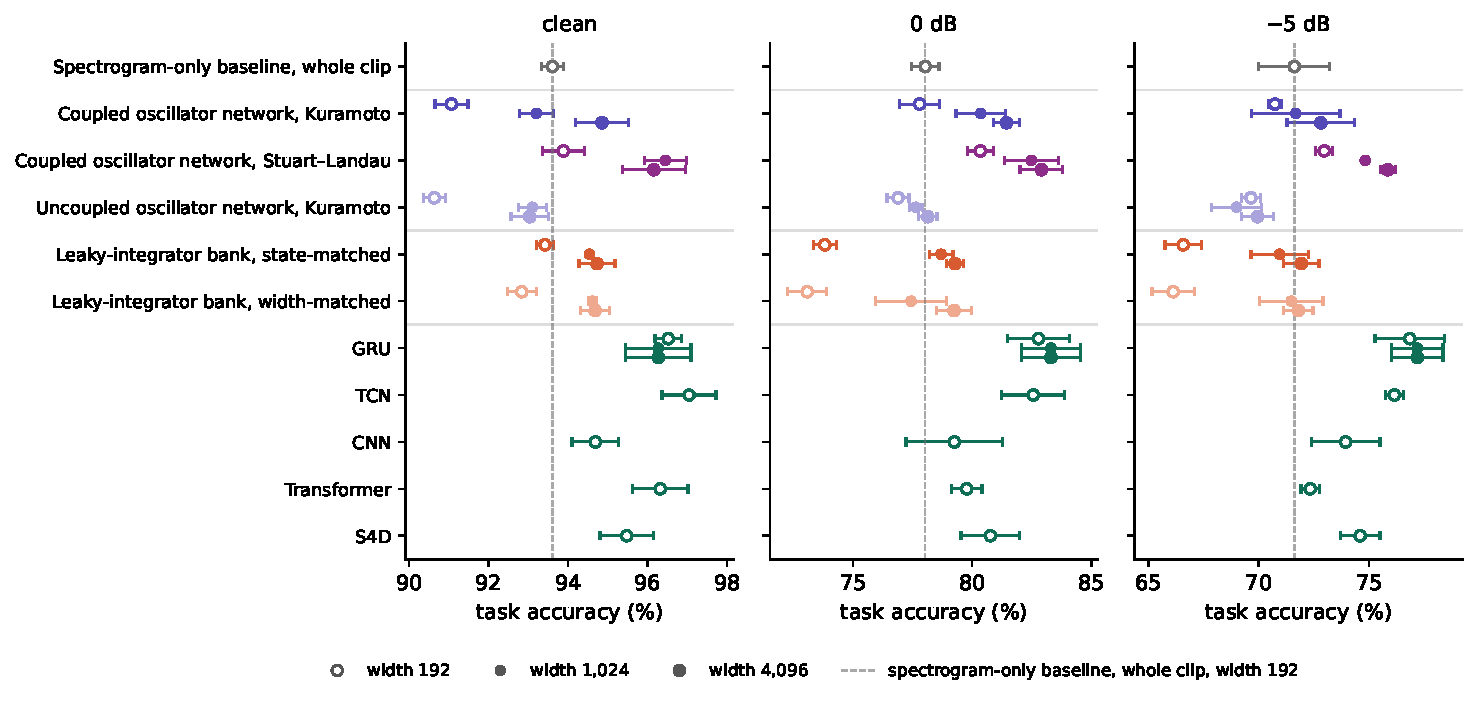
\includegraphics[keepaspectratio,alt={Recognition accuracy per arm and noise level at readout widths 192 (open circle), 1,024 (small circle) and 4,096 (square), 2,048 training clips, reservoirs at gain 1; mean  one standard deviation over three seeds. Arms no wider than 192 are read as they are, with one marker; the GRU is 216 wide. Dashed line: the whole-clip spectrogram-only baseline.}]{resources/figures/c9-readout-width.pdf}}
\caption{Recognition accuracy per arm and noise level at readout widths
192 (open circle), 1,024 (small circle) and 4,096 (square), 2,048
training clips, reservoirs at gain 1; mean \ensuremath{\pm} one standard
deviation over three seeds. Arms no wider than 192 are read as they are,
with one marker; the GRU is 216 wide. Dashed line: the whole-clip
spectrogram-only baseline.}\label{fig-c9-readout-width}
\end{figure}

\section{Discussion and conclusion}\label{sec-5}

\textbf{What the dynamics add.} Most of every arm's accuracy on the
single-digit classification task comes from the front end and the linear
readout, and the input's format matters as much: driven in quadrature,
the same networks read near chance (\hyperref[sec-4-6]{Section 4.6}).
Read directly on the spectrogram, the readout reaches 93.6\%, 78.0\% and
71.6\%, and at the common width no untrained reservoir adds more than
2.3 points to that, the most being the Stuart--Landau network's. At
gains 1 and 2 the untrained Kuramoto network does not read above its own
input. What it adds is memory: read only after its warm-up, it recovers
most of what the input loses without its first 16 frames, which hold the
onset, and it carries the order of two digits that an order-free read of
the input cannot see. A leaky-integrator bank of the same size does
both, better on order and on clean audio though about 4 points worse
with noise, and both remember by the same means, integration. A leaky
integrator keeps a running average of its band's energy; a Kuramoto
oscillator's phase advances at its natural frequency plus its drive, so,
apart from the restoring pull and the coupling, its phase is the running
sum of its band's energy wrapped around the circle. Because an
integrator's state at each moment depends on what came before it,
statistics of that state over the clip differ with the order of its
inputs, where the same statistics of the input do not. Oscillation
therefore adds no memory the bank lacks; the phase is an integrator
whose sum wraps. An analysis of variance per band and time window shows
it (\hyperref[fig-c7-anova-f]{Figure 11}; \hyperref[sec-D-2]{Appendix
D.2}): the input's class information peaks at the onset, and every
reservoir carries it into later windows. Coupling adds about a point on
noisy recognition and 2 to 19 points on order. Our results align with
the reports that much of a reservoir's accuracy comes from its front
end, for a spintronic oscillator on TI-46 \citep{abreu-araujo2020} and
for a piezoelectric reservoir on AudioMNIST, which matched logistic
regression on its input \citep{buckley2026}; its authors expect a
reservoir to help most where a linear classifier on the input falls
short, and in our noisy conditions, where it does, Kuramoto reads within
a point of the input and Stuart--Landau reads 1.1 to 2.3 points above
it.

\textbf{Network design.} A free amplitude is where the design effect
sits, not the Stuart--Landau coupling form: with its amplitude fixed,
the network reads like Kuramoto, and loses the most to a strong input.
On graphs, a Stuart--Landau network also reads above its Kuramoto
counterpart \citep{zhang2026}; fixing the amplitude, which that study
did not, places the effect in the amplitude. One reading is that a free
amplitude lets an oscillator absorb a strong drive in its radius, where
a phase oscillator can only be pushed faster. The gain sweep agrees: the
phase-oscillator networks read best at the weakest gains, and the
Stuart--Landau network near gain 1. Among phase oscillators the coupling
function and the geometry each moved accuracy by less than a point, and
a coil and a cochlea, built to follow the cochlea's shape and mechanics,
read no better than the torus.

\textbf{Readout.} With noise, more training data raised every arm, the
trained baselines three to six times as much as the Kuramoto network and
up to three times as much as the leaky-integrator banks, since in a
reservoir only the readout learns. The common width of 192 favours the
input: it reads the spectrogram's 192 features whole, but compresses a
reservoir's 12,288 to 24,576 features by 64 to 128 times through a
random projection, which keeps the distances between clips only roughly
at so few dimensions \citep{johnson1984}, so differences between digits
that the full features hold can blur. Read at 4,096, the coupled network
and the leaky-integrator banks at gain 1 pass their input, but their
readout then fits 40,970 (4,096 \ensuremath{\times} 10 digits + 10 digit
biases) weights against the 1,930 that read the input's 192 features,
about 21 times as many, so some or all of the task accuracy improvement
could come from the extra weights rather than the dynamics. The fair
comparison is at the common width, where the Kuramoto network reads
within a point of its input in noise.

\textbf{Data and training.} Many published spoken-digit results share
speakers between training and test, among them both noisy AudioMNIST
studies \citep{beoletto2026, young2026} and the TI-46 reservoirs
\citep{torrejon2017, opala2019, coulombe2017}; a classifier there, a
trained network or a readout alike, can learn the test speakers' voices,
which likely raises its accuracy, so those results are not comparable
with ours. Training is the step these results leave open, and the same
controls can say where it helps: a learned encoder before a frozen
network, a learned decoder in place of the random projection, or trained
coupling and natural frequencies, each set against the uncoupled
network, the leaky-integrator bank and the input alone at the same
number of trained parameters, would separate what the encoder, the
decoder and the oscillators learn. A trained coupled-oscillator network
reaches 89\% on AudioMNIST from the raw waveform where a plain recurrent
network fails \citep{chandravadia2026}, trained end to end on a random
split; running such a network through these controls, on held-out
speakers, would show what its oscillators contribute.

\textbf{Future directions.} The input's format decided more than the
network's design, so other formats should be tested, such as MFCCs,
cochleagrams or a cochlea-like resonator's tonogram, on which a linear
readout reached about 98\% in hardware against 75.5\% for a linear
spectrogram, with shared speakers \citep{beoletto2026}. An untrained
network needs no training and runs causally, so with a better front end
and a streaming readout it could suit low-power, real-time audio, which
our clip-pooled readout leaves untested.

\textbf{Limitations.} Three seeds give a spread but not a precise
estimate of it. The readout is one structure, a ridge on three
statistics per signal. The trained baselines are matched at about 2,000
parameters and share one training recipe rather than one tuned to each
architecture, so each might read higher with a different training
regime.

\textbf{Conclusion.} Untrained and read at a common width, a coupled
oscillator network reads about as well as its own input on noisy
speaker-disjoint spoken-digit recognition and carries the order of
events by integrating its input, as a leaky-integrator bank does;
coupling adds to both tasks, a free amplitude lifts the network above
its input in noise and a weaker input does so at 0 dB, and the lattice
geometry and phase coupling function each move it by less than a point.
Small trained networks read higher with noise, the Stuart--Landau
network alone reaching their range at gain 1, and these results are the
baseline a trained oscillator network of similar size and task should
beat.

\section*{Reproducibility statement}\label{reproducibility-statement}
\addcontentsline{toc}{section}{Reproducibility statement}

The code and the complete run record (every run's specification, results
and per-clip correctness) are in the anonymized supplementary material
and will be released with the paper; AudioMNIST is public
\citep{becker2024}. Scripts and a README with instructions on how to
reproduce the data and figures are included in the supplementary
material. Every run records its code version, hardware and library
versions. The leak check and the controls and design experiments ran on
the CPU of an Apple M1 Max, where runs with the same seed are
bit-identical. The later experiments simulated the reservoirs on its
GPU, which reproduced 1,262 of 1,296 of the controls experiment's cells
exactly and all but one within two test clips (the record's summary.md);
the trained baselines train on the CPU on every device. The experiment
harness has been set up to be able to be run on NVIDIA GPUs and Apple
Silicon in a Linux or macOS environment. We welcome reproductions.

\section*{AI use statement}\label{ai-use-statement}
\addcontentsline{toc}{section}{AI use statement}

This work was carried out by the authors working with an AI coding
agent, Claude (Anthropic), for the following purposes:

\textbf{Implementing code and tests.} Under the authors' direction the
agent wrote most of the experiment harness and the test suite. The
authors verified and independently reviewed, refactored and ran the
code.

\textbf{Refining experiments and summarizing results.} The authors set
the research questions and directed the work. The agent contributed to
flagging flaws in experimental designs, and wrote first-draft
interpretations of raw result data, which the authors reviewed and
accepted, revised or rejected.

\textbf{Drafting.} The agent drafted sections of this paper and assisted
in finding and checking correct citation format of related literature.
The authors independently verified, reviewed and revised, where
appropriate, all citations and referenced literature.

The authors take responsibility for the final content of this work.

\section*{Ethics statement}\label{ethics-statement}
\addcontentsline{toc}{section}{Ethics statement}

This work uses AudioMNIST, a public corpus of spoken digits released
under the MIT licence; we use nothing about its speakers beyond their
anonymous voice recordings, numbered by speaker so that training and
test keep speakers apart, and the audio examples in the supplementary
material are clips from it, shipped with its licence. No new data was
collected, and every experiment ran on a single Apple M1 Max computer.

\bibliography{references}
\appendix
\section*{Appendix}\label{appendix}
\addcontentsline{toc}{section}{Appendix}

\section{Glossary}\label{sec-A}

The terms as this paper uses them. The code and the run record keep
their own labels; \emph{src/README.md}, in the supplementary material,
maps each term to its label.

\subsection{The pipeline}\label{sec-A-1}

{\def\LTcaptype{none} % do not increment counter
\begin{longtable}[]{@{}
  >{\raggedright\arraybackslash}p{(\linewidth - 2\tabcolsep) * \real{0.5000}}
  >{\raggedright\arraybackslash}p{(\linewidth - 2\tabcolsep) * \real{0.5000}}@{}}
\toprule\noalign{}
\begin{minipage}[b]{\linewidth}\raggedright
Term
\end{minipage} & \begin{minipage}[b]{\linewidth}\raggedright
As used in this paper
\end{minipage} \\
\midrule\noalign{}
\endhead
\bottomrule\noalign{}
\endlastfoot
\textbf{Front end} & The fixed first stage every arm shares. It turns a
clip's 16 kHz waveform into a mel spectrogram: a 512-point Fourier
transform every 256 samples (16 ms), 16 mel bands, the log of each
band's energy, and a fixed rescaling. Nothing in it is trained or fitted
to the data. Each recording is first resampled from 48 kHz to 16 kHz,
peak-normalized, trimmed of leading and trailing silence below 1\% of
its peak and capped at 1 s. \\
\cmidrule{1-2}\textbf{Mel band} & One of the 16 frequency ranges the
front end splits the audio into, spaced on the mel scale, which follows
pitch perception: narrow at low frequencies, wide at high ones. \\
\cmidrule{1-2}\textbf{Band energy} & The log energy in one mel band, one
value per frame: the signal the front end produces for that band. \\
\cmidrule{1-2}\textbf{Mel spectrogram} & A clip's 16 band energies
together, frame by frame. The spectrogram-only baseline reads it
directly; every reservoir is driven by it. \\
\cmidrule{1-2}\textbf{Frame} & One 16 ms step of the front end, 62.5 per
second. \\
\cmidrule{1-2}\textbf{Reservoir} & An untrained dynamical system between
the front end and the readout: here the coupled and uncoupled oscillator
networks and the two leaky-integrator banks. The term is reservoir
computing's \citep{jaeger2001, maass2002}. \\
\cmidrule{1-2}\textbf{Readout} & The reader shared by every arm, and the
only fitted part of an untrained arm: one linear layer from 192 features
to 10 digit scores (1,930 weights), fitted by ridge regression, that is
least squares with an L2 penalty, solved in closed form. The penalty is
chosen from four values on the last eighth of the training clips, then
the readout is refit on all of them. It is the same for every arm, so it
is held constant across comparisons. \\
\cmidrule{1-2}\textbf{Untrained} & Parameters drawn at random once, from
the seed, and never updated. In an untrained arm only the readout is
fitted. \\
\cmidrule{1-2}\textbf{Input gain} & The factor that scales the input
before it drives a reservoir: 1 or 2. It applies only to the reservoirs:
the spectrogram-only baseline has no dynamics for it to act on, and a
trained baseline learns its own input scale. \\
\cmidrule{1-2}\textbf{Input pathway} & How the audio drives a reservoir.
Spectrogram: each band energy of the mel spectrogram adds to the
rotation rate of the oscillators in its row. Quadrature: each band's
energy and phase, so the push depends on where an oscillator is relative
to the band's own cycle, a phase-referenced drive of the kind
\citet{adler1946} analysed. \\
\end{longtable}
}

\subsection{Arms and baselines}\label{sec-A-2}

{\def\LTcaptype{none} % do not increment counter
\begin{longtable}[]{@{}
  >{\raggedright\arraybackslash}p{(\linewidth - 2\tabcolsep) * \real{0.5000}}
  >{\raggedright\arraybackslash}p{(\linewidth - 2\tabcolsep) * \real{0.5000}}@{}}
\toprule\noalign{}
\begin{minipage}[b]{\linewidth}\raggedright
Term
\end{minipage} & \begin{minipage}[b]{\linewidth}\raggedright
As used in this paper
\end{minipage} \\
\midrule\noalign{}
\endhead
\bottomrule\noalign{}
\endlastfoot
\textbf{Arm} & One system under comparison, read the same way as every
other. The term comes from experimental design. \\
\cmidrule{1-2}\textbf{Spectrogram-only baseline} & The front end and the
readout with nothing between them: the readout reads the band energies
directly, so it measures what the input alone supports. Read from the
first frame, over the whole clip, it is the primary control, because it
sees everything a reservoir is driven with; read from frame 16, it sees
the frames every other arm is read over. On the quadrature pathway it
reads that pathway's front end instead. \\
\cmidrule{1-2}\textbf{Coupled oscillator network} & The system under
test: 1,024 untrained oscillators in 4 channels of a 16
\ensuremath{\times} 16 lattice, coupled within each channel through a
coupling kernel, with 2,048 parameters (the kernels and the natural
frequencies). Also ``the oscillator network''. Its reference
configuration: Kuramoto coupling, torus geometry, random natural
frequencies, restoring strength 0.3, coupling ceiling 1. \\
\cmidrule{1-2}\textbf{Uncoupled oscillator network} & The same network
with every coupling kernel set to zero: each oscillator keeps its
natural frequency, restoring strength and input, but none acts on
another. It isolates what the coupling contributes. \\
\cmidrule{1-2}\textbf{Leaky integrator} & A unit that holds one number x
and, at each frame, moves a fraction a of the way toward its input: x
\ensuremath{\leftarrow} (1 \ensuremath{-} a)\ensuremath{\cdot}x +
a\ensuremath{\cdot}tanh(g\_in\ensuremath{\cdot}g\ensuremath{\cdot}u),
where u is the input, g the input gain, g\_in the unit's own input
weight, and \(\tanh\) bounds the input. The old value decays
exponentially, or ``leaks'', so the unit is a running average of its
recent input with a time constant set by a; in signal-processing terms
it is a first-order low-pass filter. The term is standard. In
computational neuroscience it is the leaky-integrator neuron, the leaky
integrate-and-fire model without the firing; in reservoir computing it
is the unit of leaky-integrator echo state networks \citep{jaeger2007},
whose a is the ``leaking rate'' \citep{lukosevicius2012}. \\
\cmidrule{1-2}\textbf{Leaky-integrator bank} & A reservoir of
independent leaky integrators, routed like the oscillator network: mel
band r drives every unit in row r. Time constants are spaced
logarithmically from 16 ms to 1 s, input weights g\_in are drawn with
mean 1 and standard deviation 0.1, and no unit is connected to another:
nothing rotates and nothing is coupled. State-matched: 1,024 units, the
oscillator network's number of states and parameters. Width-matched:
2,048 units, the number of signals the oscillator network exposes (sin
\ensuremath{\theta} and cos \ensuremath{\theta} of each oscillator), at
twice the parameters. \\
\cmidrule{1-2}\textbf{Trained baselines} & Five conventional networks of
1,840 to 2,109 parameters, trained end to end (AdamW, 30 epochs) through
a learned linear layer on the same statistics, standardized, then read
by the same readout. GRU: a gated recurrent network. TCN: a temporal
convolutional network, two residual blocks of dilated causal
convolutions (receptive field 31 frames). CNN: two causal
one-dimensional convolutions (receptive field 9 frames). Transformer:
one causal self-attention layer, width 16 with two heads, and a
two-layer feed-forward block. S4D: a diagonal state-space model, its
time constants initialized from 2 to 200 frames. \\
\cmidrule{1-2}\textbf{Matched pair} & Two runs identical in every factor
but the one compared, at the same noise level, input gain and seed. A
design factor's effect is the mean difference over its matched pairs. \\
\cmidrule{1-2}\textbf{Seed} & Sets an arm's random parameters and which
training clips it draws. Every condition is run at three seeds, and
results are reported as their mean with the standard deviation. \\
\end{longtable}
}

\subsection{The oscillator network}\label{sec-A-3}

{\def\LTcaptype{none} % do not increment counter
\begin{longtable}[]{@{}
  >{\raggedright\arraybackslash}p{(\linewidth - 2\tabcolsep) * \real{0.5000}}
  >{\raggedright\arraybackslash}p{(\linewidth - 2\tabcolsep) * \real{0.5000}}@{}}
\toprule\noalign{}
\begin{minipage}[b]{\linewidth}\raggedright
Term
\end{minipage} & \begin{minipage}[b]{\linewidth}\raggedright
As used in this paper
\end{minipage} \\
\midrule\noalign{}
\endhead
\bottomrule\noalign{}
\endlastfoot
\textbf{Oscillator} & A unit whose state advances around a cycle. A
phase oscillator keeps only its phase \ensuremath{\theta}, an angle; a
Stuart--Landau oscillator also keeps an amplitude. The readout sees sin
\ensuremath{\theta} and cos \ensuremath{\theta} of each. \\
\cmidrule{1-2}\textbf{Natural frequency \ensuremath{\omega}} & The rate
at which an oscillator would advance if nothing acted on it: random, the
reference, tonotopic or identical (\hyperref[sec-4-4]{Section 4.4}). \\
\cmidrule{1-2}\textbf{Lattice} & The 16 \ensuremath{\times} 16 grid a
channel's oscillators sit on. Rows follow frequency: mel band r drives
row r, from lowest to highest. \\
\cmidrule{1-2}\textbf{Lattice geometry} & Which oscillators of a channel
are neighbours, that is, how the lattice's edges are glued: torus,
cylinder, sheet, helix, cube, sphere, coil or cochlea
(\hyperref[sec-C]{Appendix C}). \\
\cmidrule{1-2}\textbf{Row} & The 16 oscillators of one channel that a
single mel band drives. The only grouping built into the network. \\
\cmidrule{1-2}\textbf{Channel} & One independent 16 \ensuremath{\times}
16 lattice of 256 oscillators, with its own coupling kernel and natural
frequencies. Every channel receives the same input, and channels do not
act on each other; the network's 4 channels are four differently drawn
copies, read side by side. The name follows the channels of a
convolutional network, where each channel likewise has its own
kernel. \\
\cmidrule{1-2}\textbf{Coupling kernel} & A channel's table of coupling
weights: a 16 \ensuremath{\times} 16 array whose entry at an offset of
so many rows and columns sets how strongly an oscillator is acted on by
the one at that offset. The same table applies at every site, so the
coupling is a convolution, and ``kernel'' is meant as in a convolutional
network, not as a GPU compute kernel. It covers every offset, so each
oscillator is coupled to every other in its channel. The weights are
drawn from N(0, 0.05\ensuremath{^{2}}): a positive weight pulls a pair
toward the same phase, a negative one pushes it apart. Each channel has
its own kernel. \\
\cmidrule{1-2}\textbf{Coupling function} & How the phases of two coupled
oscillators turn into a push on one of them (\hyperref[sec-B]{Appendix
B}). \\
\cmidrule{1-2}\textbf{Coupling ceiling} & A cap on each channel's
overall coupling strength, 1 or 0.5. It limits the channel's coupling as
a whole, the largest factor by which the kernel amplifies any spatial
pattern of phases across the channel (the peak of the kernel's
spectrum), and enforces it by scaling every weight of that channel's
kernel by the same factor. It does not cap individual pairs, neighbours
or regions. Random kernels always exceed it here (peaks of 1.4 to 2.9 on
the torus), so in practice the ceiling sets every channel's coupling
strength. \\
\cmidrule{1-2}\textbf{Restoring strength \ensuremath{\lambda}} & The
strength of a pull on every oscillator back toward phase 0, the term
\ensuremath{-\lambda} sin \ensuremath{\theta}, 0.3 or 0.1. It has the
form of the restoring torque that returns a pendulum to rest, but the
oscillators have no inertia, so nothing swings back past 0: an
oscillator whose natural frequency is below \ensuremath{\lambda} is held
in place, or locked \citep{adler1946}, and a faster one keeps rotating,
slowed where the pull opposes it. For Stuart--Landau oscillators it is a
pull toward phase 0 at unit amplitude. \\
\cmidrule{1-2}\textbf{Cluster} & A group of oscillators that move
together, in phase or in fixed opposition, because of the dynamics
rather than the wiring. Nothing in a kernel assigns an oscillator to a
cluster; clusters form, or do not, as the network runs
\citep{pikovsky2001}. \\
\cmidrule{1-2}\textbf{Rotation rate} & How far an oscillator's phase
advances between frames. The spectrogram pathway adds each band energy
to it. \\
\end{longtable}
}

\subsection{The read and the evaluation}\label{sec-A-4}

{\def\LTcaptype{none} % do not increment counter
\begin{longtable}[]{@{}
  >{\raggedright\arraybackslash}p{(\linewidth - 2\tabcolsep) * \real{0.5000}}
  >{\raggedright\arraybackslash}p{(\linewidth - 2\tabcolsep) * \real{0.5000}}@{}}
\toprule\noalign{}
\begin{minipage}[b]{\linewidth}\raggedright
Term
\end{minipage} & \begin{minipage}[b]{\linewidth}\raggedright
As used in this paper
\end{minipage} \\
\midrule\noalign{}
\endhead
\bottomrule\noalign{}
\endlastfoot
\textbf{Signal} & A time series an arm exposes to the readout: a band
energy for the spectrogram-only baseline, sin \ensuremath{\theta} or cos
\ensuremath{\theta} of an oscillator, a leaky integrator's state, or a
trained baseline's hidden unit. \\
\cmidrule{1-2}\textbf{Summary statistics} & Per signal and window: the
mean, the standard deviation and the mean absolute frame-to-frame
change. None is an endpoint, and the absolute change cannot tell a
rising signal from a falling one. \\
\cmidrule{1-2}\textbf{Window} & For recognition, frames 16 to 61 split
into four equal windows; for the order task, frames 16 to 147 as one.
Every clip is read over the same frames. \\
\cmidrule{1-2}\textbf{Warm-up} & The first 16 frames (256 ms), which
every arm but the whole-clip spectrogram-only baseline skips. Reading
every arm over the same frames after the warm-up means an arm with no
input reads chance. \\
\cmidrule{1-2}\textbf{Width} & The number of features the readout sees:
192, 1,024 or 4,096. An arm with more features than that is projected
down to it by a random Gaussian matrix, the fixed draw or one drawn for
each run seed; one with fewer is read as it is
(\hyperref[sec-3-3]{Section 3.3}). An arm's native width is its feature
count before projection: 192 for the spectrogram-only baseline, 24,576
for the oscillator network. \\
\cmidrule{1-2}\textbf{Primary cell} & Width 192, 2,048 training clips,
and the four-window read (the whole-span read for the order task). \\
\cmidrule{1-2}\textbf{Protocols A and B} & A: train on speakers 1 to 48
and test on the 6,000 clips of speakers 49 to 60. B: the five speaker
folds of \citet{becker2024}. \\
\cmidrule{1-2}\textbf{Noise level} & White noise added to each clip at a
level set by its speech, given as the signal-to-noise ratio: at 0 dB the
noise is as loud as the speech, and at \ensuremath{-}5 dB it is 5 dB
louder. Each clip's noise comes from a generator seeded by the clip, so
every arm hears the same noisy clip. \\
\cmidrule{1-2}\textbf{Order task} & Two digits of a pair spoken one
after the other; the task is to say which came first. The mean and
spread of a signal do not depend on the order of its frames, so the
input alone read over the whole span cannot answer it, and the
spectrogram-only baseline reads chance, 50\%. Each pair has 2,048
training sequences from the training speakers and 2,048 test sequences
from the test speakers, balanced between the two orders. \\
\end{longtable}
}

\section{Coupling functions}\label{sec-B}

Each oscillator's phase \ensuremath{\theta_{i}} evolves as
\ensuremath{\dot{\theta}_{i}} = \ensuremath{\omega_{i}} +
coupling\ensuremath{_{i}} + g\ensuremath{\cdot}u\ensuremath{_{i}}
\ensuremath{-} \ensuremath{\lambda} sin \ensuremath{\theta_{i}}: its
natural frequency, the coupling from the other oscillators of its
channel, the input and a restoring pull toward phase 0. The six coupling
functions differ only in the coupling term. Four are phase models that
machine-learning systems have built on or that physics offers as
controlled departures from Kuramoto's; two are Stuart--Landau
amplitude-phase oscillators, with and without their amplitude. A recent
survey found coupling functions compared under controls only within the
Kuramoto family, in FSN \citep{nunley2026}, and called the choice
between families ``a convention rather than a finding''
\citep{kryski2026}; one graph network sets Stuart--Landau against
Kuramoto and reads above it, but does not fix the amplitude
\citep{zhang2026}. \hyperref[fig-a3-coupling-functions]{Figure 8}
illustrates how each pushes an oscillator.

\begin{longtable}[]{@{}
  >{\raggedright\arraybackslash}p{(\linewidth - 6\tabcolsep) * \real{0.2500}}
  >{\raggedright\arraybackslash}p{(\linewidth - 6\tabcolsep) * \real{0.2500}}
  >{\raggedright\arraybackslash}p{(\linewidth - 6\tabcolsep) * \real{0.2500}}
  >{\raggedright\arraybackslash}p{(\linewidth - 6\tabcolsep) * \real{0.2500}}@{}}
\caption{The six coupling functions. K\ensuremath{_{ij}} is the kernel
weight between oscillators i and j, positive or negative, and each term
is summed over the other oscillators of the channel. Machine-learning
uses are those recorded by the survey of
\citet{kryski2026}.}\tabularnewline
\toprule\noalign{}
\begin{minipage}[b]{\linewidth}\raggedright
coupling function
\end{minipage} & \begin{minipage}[b]{\linewidth}\raggedright
coupling term
\end{minipage} & \begin{minipage}[b]{\linewidth}\raggedright
what it adds
\end{minipage} & \begin{minipage}[b]{\linewidth}\raggedright
in machine learning
\end{minipage} \\
\midrule\noalign{}
\endfirsthead
\toprule\noalign{}
\begin{minipage}[b]{\linewidth}\raggedright
coupling function
\end{minipage} & \begin{minipage}[b]{\linewidth}\raggedright
coupling term
\end{minipage} & \begin{minipage}[b]{\linewidth}\raggedright
what it adds
\end{minipage} & \begin{minipage}[b]{\linewidth}\raggedright
in machine learning
\end{minipage} \\
\midrule\noalign{}
\endhead
\bottomrule\noalign{}
\endlastfoot
\textbf{Kuramoto} & \ensuremath{\Sigma_{j}} K\ensuremath{_{ij}}
sin(\ensuremath{\theta_{j}} \ensuremath{-} \ensuremath{\theta_{i}}) &
pulls each oscillator toward the others' phases: the minimal model of
synchronization \citep{kuramoto1975}, and the reference & trained
all-to-all in Un-0 \citep{unconv-ai2026}; a D-dimensional generalization
in AKOrN \citep{miyato2025} \\
\cmidrule{1-4}\textbf{Kuramoto--Sakaguchi} & \ensuremath{\Sigma_{j}}
K\ensuremath{_{ij}} sin(\ensuremath{\theta_{j}} \ensuremath{-}
\ensuremath{\theta_{i}} \ensuremath{-} \ensuremath{\alpha}),
\ensuremath{\alpha} = \ensuremath{\pi}/4 & a phase lag that breaks the
pull's symmetry and admits partial coherence
\citep{sakaguchi1986, abrams2004} & with Daido harmonics and a delay in
FSN \citep{nunley2026} \\
\cmidrule{1-4}\textbf{Second harmonic} & Kuramoto plus
\ensuremath{\beta} \ensuremath{\Sigma_{j}} K\ensuremath{_{ij}} sin
2(\ensuremath{\theta_{j}} \ensuremath{-} \ensuremath{\theta_{i}}),
\ensuremath{\beta} = 0.5 & favours two-cluster states, pairs in phase or
in opposition \citep{daido1992, hansel1993} & among FSN's Daido
harmonics \citep{nunley2026} \\
\cmidrule{1-4}\textbf{Winfree} & \ensuremath{-}sin
\ensuremath{\theta_{i}} \ensuremath{\Sigma_{j}} K\ensuremath{_{ij}} (1 +
cos \ensuremath{\theta_{j}}) & separates an oscillator's sensitivity,
set by its own phase, from its influence, set by its neighbour's
\citep{winfree1967} & generalized, with attention-defined coupling, in
WONN \citep{dai2026} \\
\cmidrule{1-4}\textbf{Stuart--Landau} & \ensuremath{\Sigma_{j}}
K\ensuremath{_{ij}} (z\ensuremath{_{j}} \ensuremath{-}
z\ensuremath{_{i}}), z = x + iy & amplitude as well as phase: each
oscillator relaxes to a cycle of unit radius
\citep{stuart1960, aranson2002} & one graph network \citep{zhang2026} \\
\cmidrule{1-4}\textbf{Stuart--Landau, fixed amplitude} & the same,
amplitude held at 1 & the phase-only limit, which reduces to Kuramoto:
separates what the amplitude adds & none recorded \\
\end{longtable}

\begin{figure}
\centering
\pandocbounded{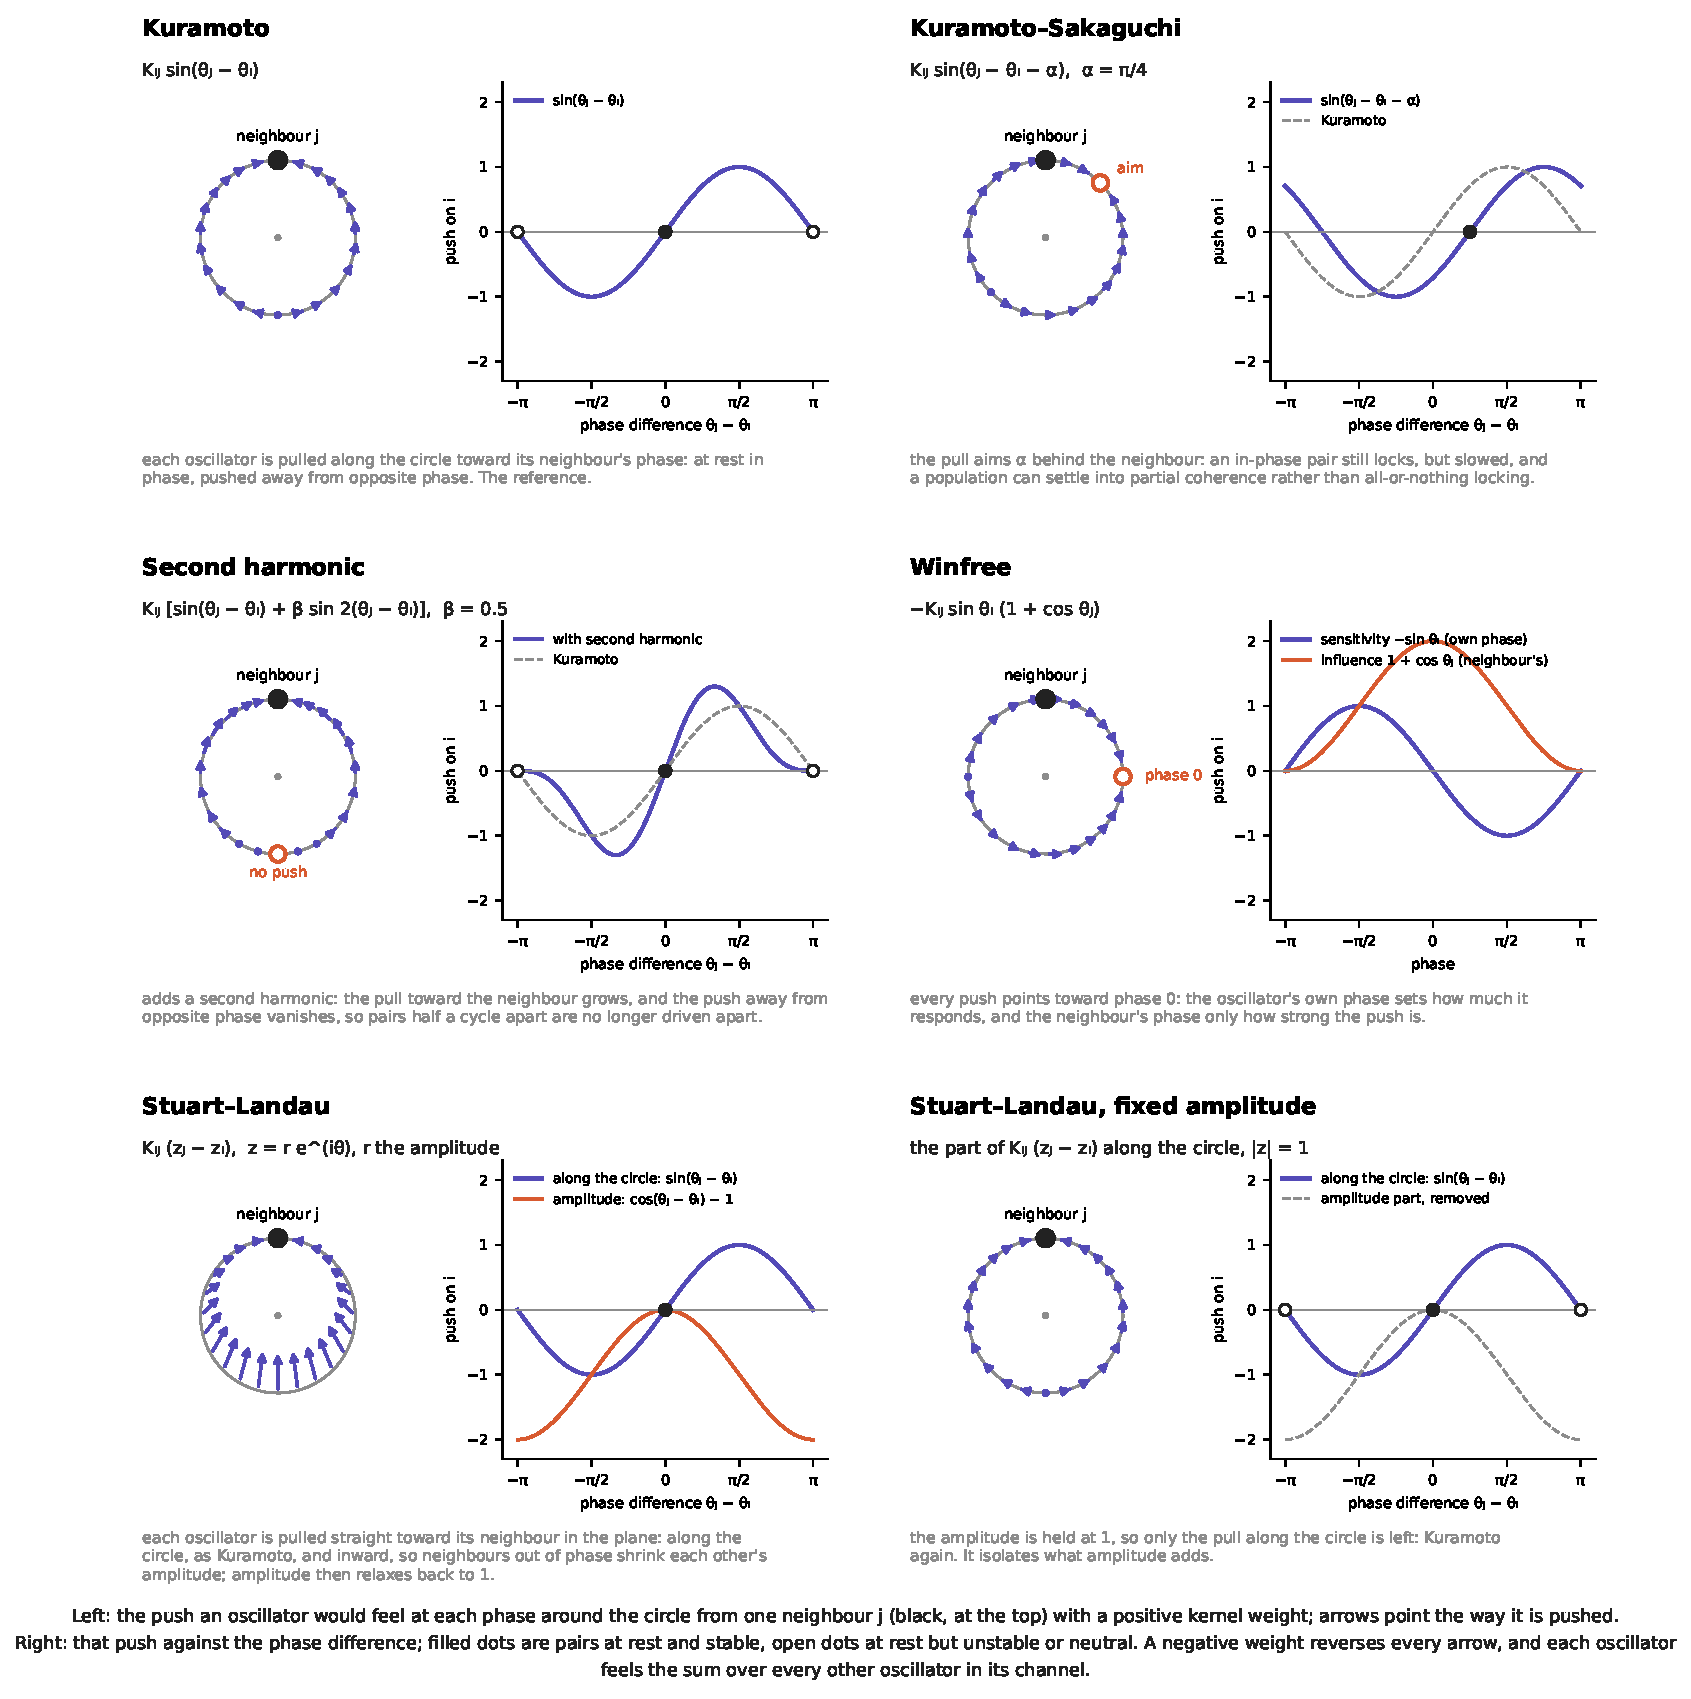
\includegraphics[keepaspectratio,alt={Coupling functions, for one neighbour j with a positive kernel weight. Left: the push on an oscillator at each phase while j sits at the top (arrows). Right: that push against   ; filled dots, stable rest; open dots, unstable or neutral. Kuramoto pulls toward the neighbour; Kuramoto--Sakaguchi aims  = /4 behind it; the second harmonic ( = 0.5) strengthens the pull and removes the push away from opposite phase; Winfree pushes toward phase 0, the neighbour setting only how hard; Stuart--Landau pulls straight toward the neighbour in the plane, so out-of-phase neighbours shrink each other's amplitude, and at fixed amplitude it reduces to Kuramoto. A negative weight reverses every arrow.}]{resources/figures/a3-coupling-functions.pdf}}
\caption{Coupling functions, for one neighbour j with a positive kernel
weight. Left: the push on an oscillator at each phase while j sits at
the top (arrows). Right: that push against \ensuremath{\theta_{j}}
\ensuremath{-} \ensuremath{\theta_{i}}; filled dots, stable rest; open
dots, unstable or neutral. Kuramoto pulls toward the neighbour;
Kuramoto--Sakaguchi aims \ensuremath{\alpha} = \ensuremath{\pi}/4 behind
it; the second harmonic (\ensuremath{\beta} = 0.5) strengthens the pull
and removes the push away from opposite phase; Winfree pushes toward
phase 0, the neighbour setting only how hard; Stuart--Landau pulls
straight toward the neighbour in the plane, so out-of-phase neighbours
shrink each other's amplitude, and at fixed amplitude it reduces to
Kuramoto. A negative weight reverses every
arrow.}\label{fig-a3-coupling-functions}
\end{figure}

\section{Lattice geometries}\label{sec-C}

In our experiment, every channel stores its 256 oscillators as a 16
\ensuremath{\times} 16 grid whose row r is driven by mel band r. A
lattice geometry changes only which oscillators are neighbours, that is,
how the grid's edges are glued; each of a network's four channels is a
separate copy of the same shape, and the kernel, the parameters and the
oscillators are the same under every geometry, so a comparison between
geometries varies one thing. The torus is the reference every other
geometry is compared against. Wrapped in both directions, it has no
edges, so every oscillator has the same neighbourhood and no position in
the lattice is special, and each other geometry departs from it in one
respect: opening edges, adding a dimension, or laying frequency out
differently. Here no geometry read above it by more than 0.21 points
(\hyperref[sec-4-4]{Section 4.4}).

\begin{longtable}[]{@{}
  >{\raggedright\arraybackslash}p{(\linewidth - 2\tabcolsep) * \real{0.5000}}
  >{\raggedright\arraybackslash}p{(\linewidth - 2\tabcolsep) * \real{0.5000}}@{}}
\caption{The eight lattice geometries. The first six run in the design
experiment; the coil and the cochlea in the cochlea
experiment.}\tabularnewline
\toprule\noalign{}
\begin{minipage}[b]{\linewidth}\raggedright
Geometry
\end{minipage} & \begin{minipage}[b]{\linewidth}\raggedright
How the grid is shaped
\end{minipage} \\
\midrule\noalign{}
\endfirsthead
\toprule\noalign{}
\begin{minipage}[b]{\linewidth}\raggedright
Geometry
\end{minipage} & \begin{minipage}[b]{\linewidth}\raggedright
How the grid is shaped
\end{minipage} \\
\midrule\noalign{}
\endhead
\bottomrule\noalign{}
\endlastfoot
\textbf{Torus} & Both axes wrap: the top row is coupled to the bottom,
and the left column to the right. The reference geometry. \\
\cmidrule{1-2}\textbf{Cylinder} & Columns wrap, rows do not: the
frequency axis is open, as in the cochlea, so the highest band is not
coupled around to the lowest. \\
\cmidrule{1-2}\textbf{Sheet} & Neither axis wraps, and coupling stops at
every edge. With the cylinder and the torus it varies the number of
wrapped axes from zero to two. \\
\cmidrule{1-2}\textbf{Helix} & The 256 sites read as one closed ring,
one octave (64 sites, four rows) per turn, so an offset of one turn
joins bands an octave apart. \\
\cmidrule{1-2}\textbf{Cube} & Each row's 16 columns read as a 4
\ensuremath{\times} 4 slab, giving a 16 \ensuremath{\times} 4
\ensuremath{\times} 4 lattice that wraps on all three axes: the same
oscillators, with shorter paths between them. \\
\cmidrule{1-2}\textbf{Sphere} & Rows as latitudes with open poles and
columns as longitudes that wrap, each oscillator's influence weighted by
the cosine of its latitude: an approximation to a sphere, not exact
spherical coupling. \\
\cmidrule{1-2}\textbf{Coil} & The 256 sites read as one open line from
the base (highest band) to the apex (lowest band), one octave per turn:
the helix with its ends apart, as the cochlea's spiral is open at both
ends, so an offset of one turn joins sites that sit side by side on
adjacent turns. \\
\cmidrule{1-2}\textbf{Cochlea} & The coil with two features of the
cochlea's mechanics: influence runs three times as strongly from base to
apex as back, as the travelling wave does, and the coupling into each
site grows with the coil's curvature, from a quarter at the base to full
strength at the apex, as the spiral tightens. A control keeps both at
the coil's average coupling. \\
\end{longtable}

The first six vary the number of wrapped axes (sheet, cylinder, torus),
the dimension (the cube, which shortens the paths between oscillators)
and how frequency is laid out: the cylinder and the sphere leave the
frequency axis open, as the cochlea does, and the helix puts bands an
octave apart next to each other, as the pitch helix of music perception
does \citep{shepard1982}. The helix is not a cochlea: it is closed, and
nothing in it runs one way. The coil and the cochlea follow the cochlea
itself, whose coiled, tonotopic shape a spiral metamaterial resonator
has used to classify AudioMNIST digits \citep{beoletto2026}; with
tonotopic natural frequencies, each coil position's frequency falls
exponentially from base to apex, as along the basilar membrane.
Oscillator lattices are a long-studied setting in physics
\citep{sakaguchi1987}, and machine-learning systems couple oscillators
all-to-all \citep{unconv-ai2026}, through attention, or locally on a
lattice \citep{keller2023, miyato2025}. Geometry has been varied in
several of the systems the survey covers, ``and in none of them as a
single variable'', and it found no work that varies coupling range or
boundary conditions at a matched budget \citep{kryski2026}.

\begin{figure}
\centering
\pandocbounded{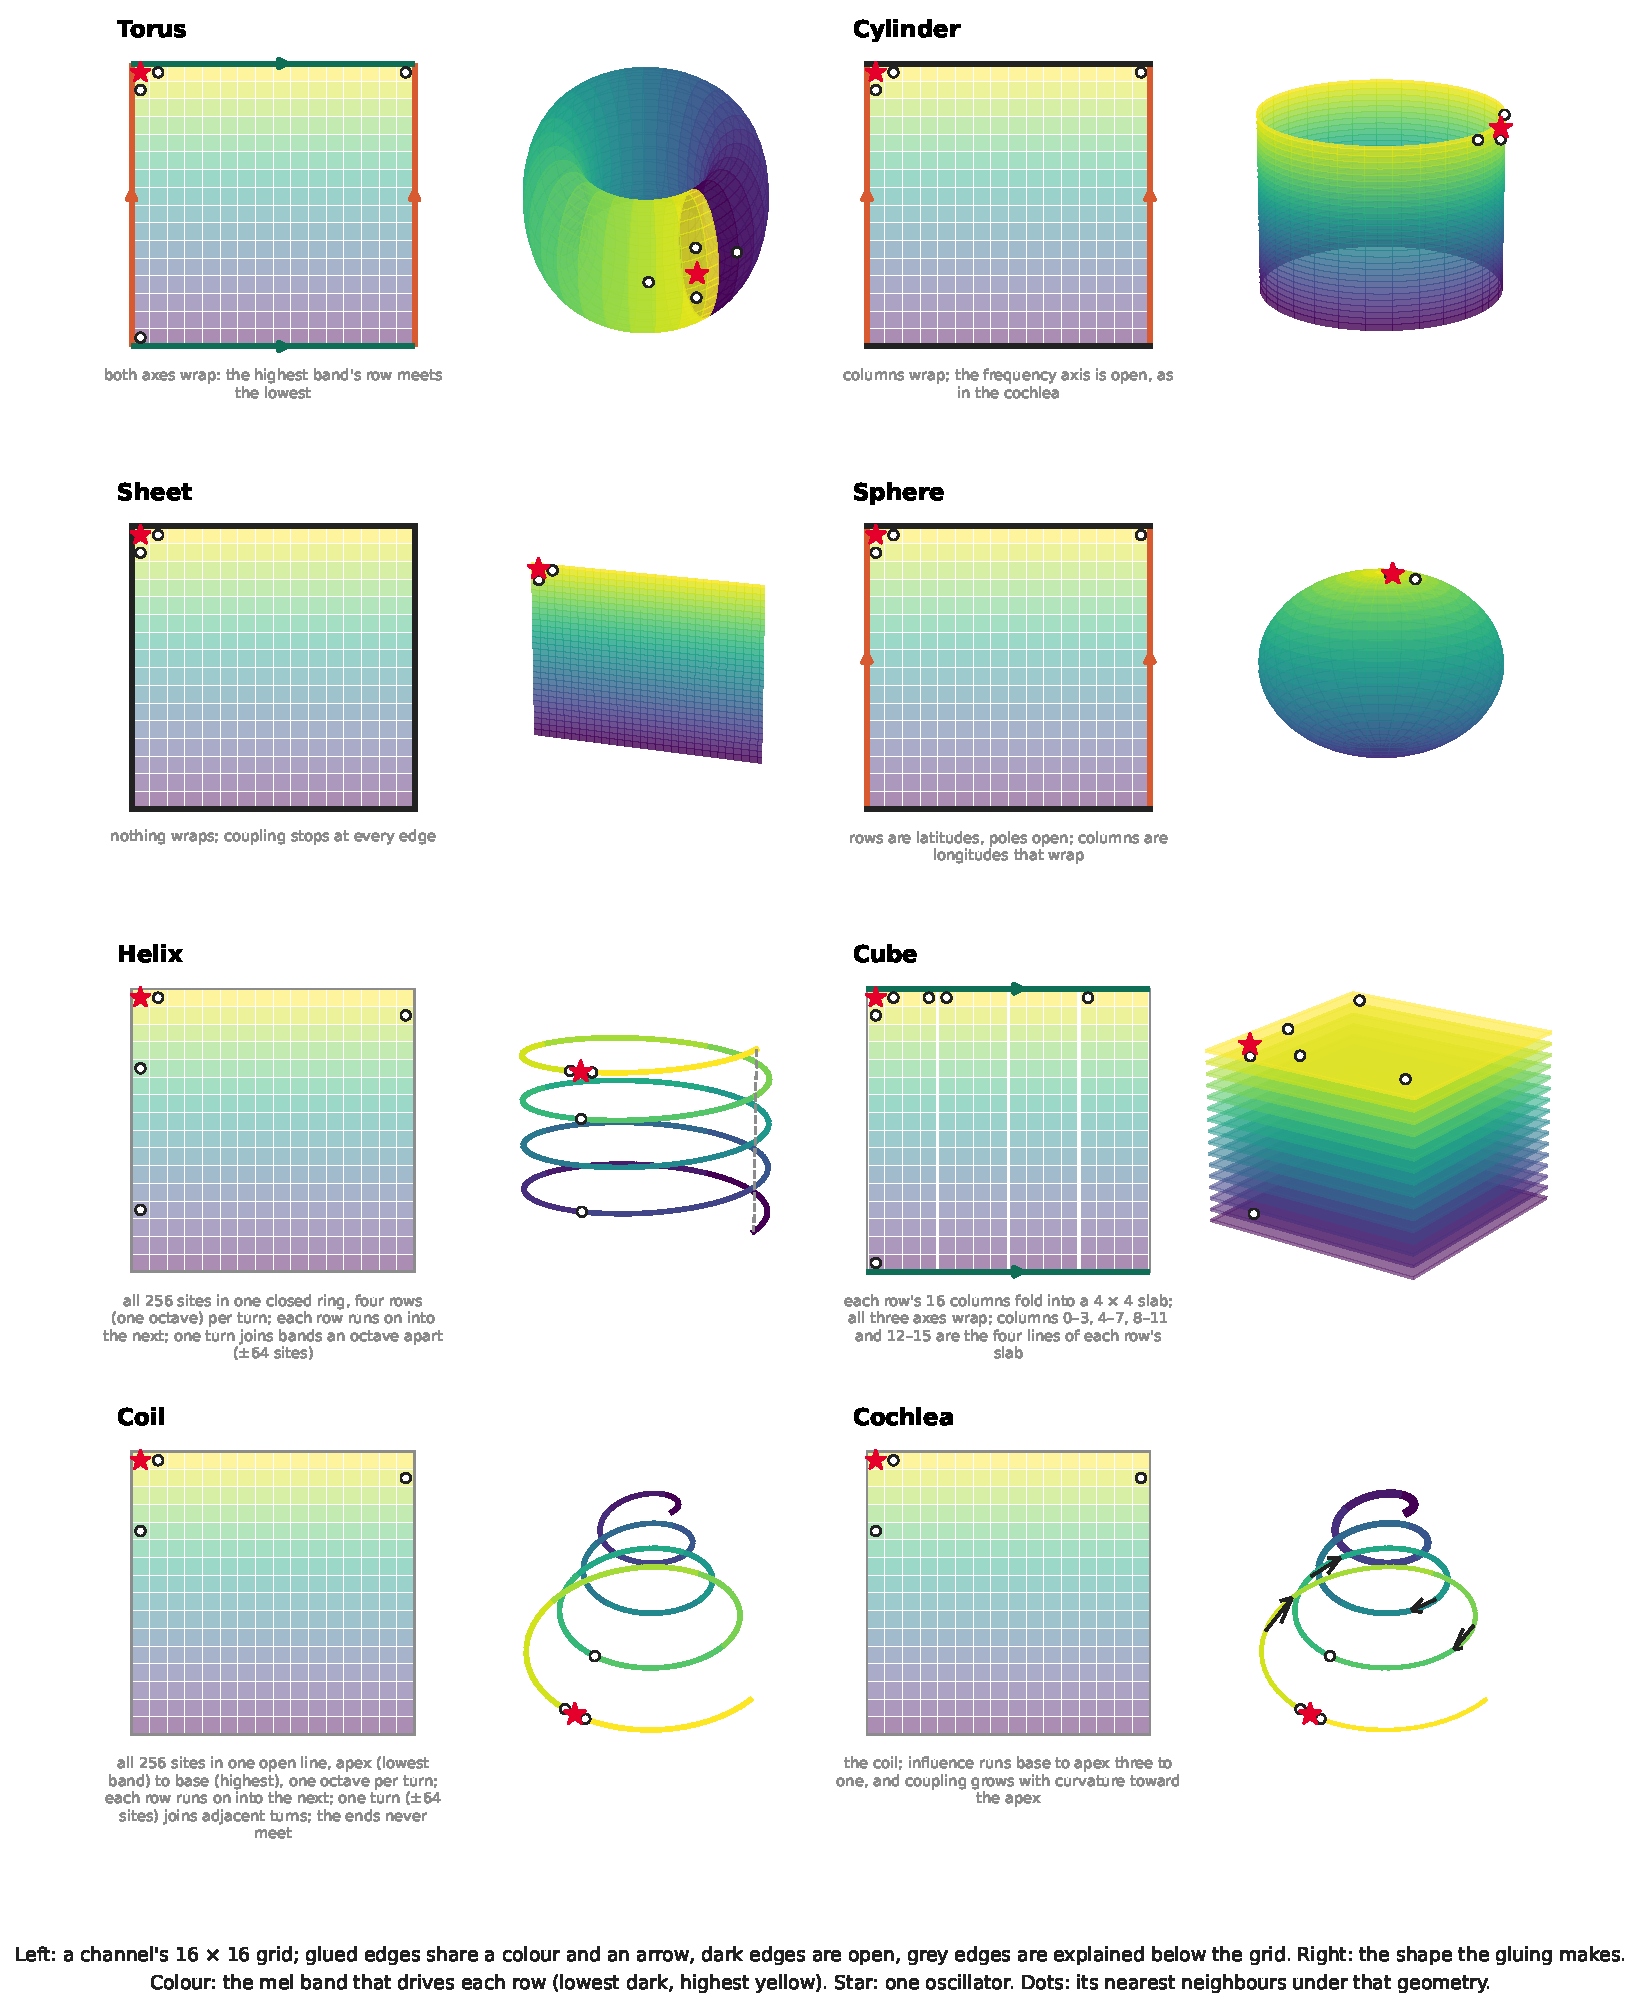
\includegraphics[keepaspectratio,alt={Lattice geometries. Each channel is a 16  16 grid whose row r is driven by mel band r (colour, lowest band dark); a geometry changes only how the grid's edges are glued. Left: the grid, glued edges marked by a shared colour and arrow, open edges dark, one oscillator (star) and its nearest neighbours (dots); right: the shape this makes. The torus joins the highest band's row to the lowest; the cylinder and the sphere leave the frequency axis open; the helix threads the 256 sites into one closed ring, an octave per turn; the cube folds each row into a 4  4 slab and wraps all three axes; the coil threads them into one open line, apex (lowest band) at the centre; the cochlea adds the base-to-apex direction (arrows) and coupling that grows toward the apex (thicker line).}]{resources/figures/a2-lattice-geometries.pdf}}
\caption{Lattice geometries. Each channel is a 16 \ensuremath{\times} 16
grid whose row r is driven by mel band r (colour, lowest band dark); a
geometry changes only how the grid's edges are glued. Left: the grid,
glued edges marked by a shared colour and arrow, open edges dark, one
oscillator (star) and its nearest neighbours (dots); right: the shape
this makes. The torus joins the highest band's row to the lowest; the
cylinder and the sphere leave the frequency axis open; the helix threads
the 256 sites into one closed ring, an octave per turn; the cube folds
each row into a 4 \ensuremath{\times} 4 slab and wraps all three axes;
the coil threads them into one open line, apex (lowest band) at the
centre; the cochlea adds the base-to-apex direction (arrows) and
coupling that grows toward the apex (thicker
line).}\label{fig-a2-lattice-geometries}
\end{figure}

\section{The readout}\label{sec-D}

\subsection{The readout for each arm}\label{sec-D-1}

\begin{figure}
\centering
\pandocbounded{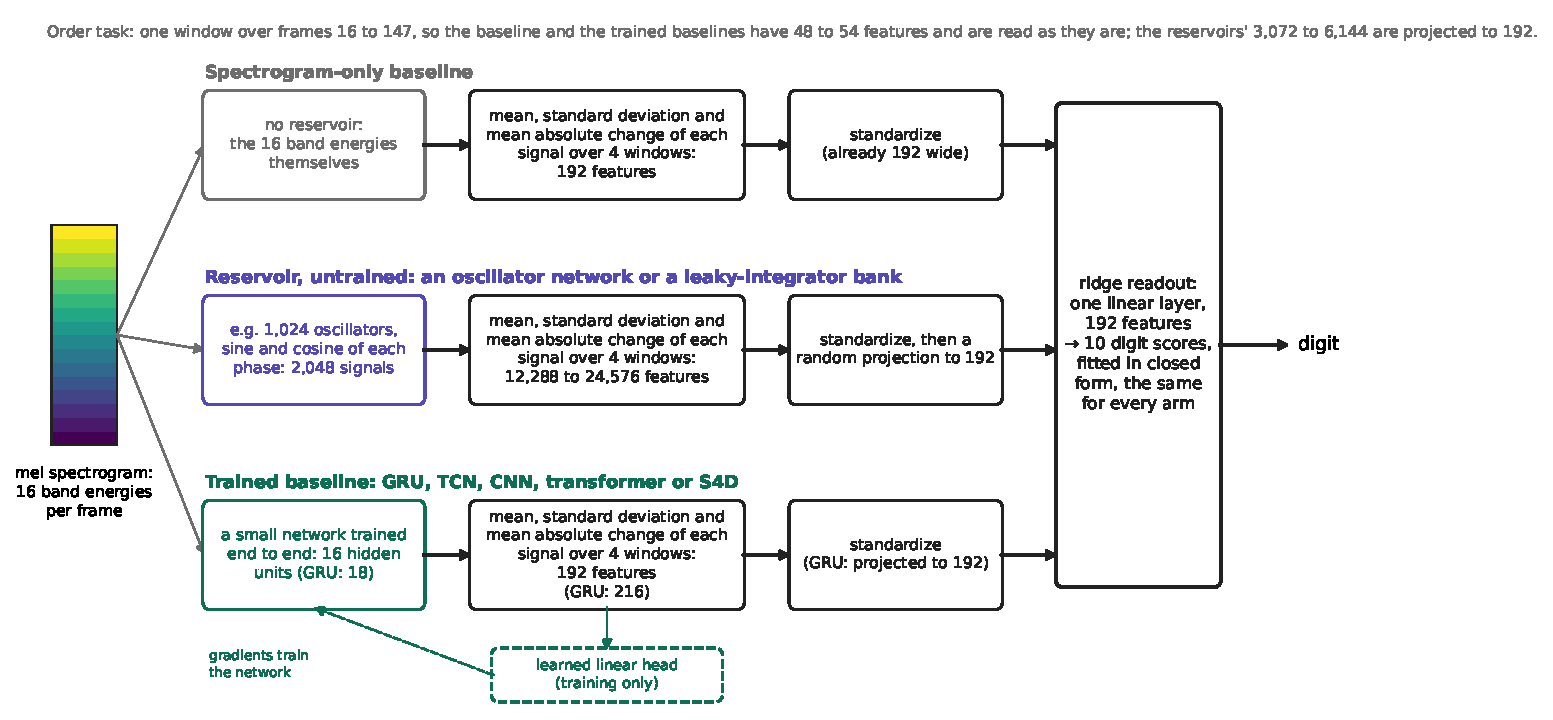
\includegraphics[keepaspectratio,alt={The readout for each kind of arm: the same three statistics over the same four windows, classified by a ridge readout fitted to each arm. The spectrogram-only baseline's 192 features are read as they are; a reservoir's 12,288 to 24,576 are standardized and projected to 192 by a fixed random matrix; a trained baseline's 192 (the GRU's 216, projected) are read after the network is trained end to end through a learned linear head.}]{resources/figures/a4-the-read.pdf}}
\caption{The readout for each kind of arm: the same three statistics
over the same four windows, classified by a ridge readout fitted to each
arm. The spectrogram-only baseline's 192 features are read as they are;
a reservoir's 12,288 to 24,576 are standardized and projected to 192 by
a fixed random matrix; a trained baseline's 192 (the GRU's 216,
projected) are read after the network is trained end to end through a
learned linear head.}\label{fig-a4-the-read}
\end{figure}

\subsection{Where each arm carries class information}\label{sec-D-2}

Following \citet{beoletto2026}, a one-way analysis of variance measures
where in time and frequency each arm carries information about the
digit. Every signal of an arm is averaged over each sixteenth of the
padded clip (frames 0 to 61, warm-up included, so the input's onset
shows), and each average is tested for a difference between the ten
digits over the 2,048 training clips of seed 0 at 0 dB (gain 1 for the
reservoirs); F is the variance between digits over the variance within
them, each over its degrees of freedom. The maps average F over the
signals of each mel band: the band itself for the spectrogram, and the
sine and cosine of every oscillator, or every integrator's state, in
that band's row, over channels and columns. They describe where the
information sits; they do not compare accuracy.

The input carries its information in a burst at the onset: its F peaks
at 425 in band 4 in the fourth window, and averages 119 over windows 7
to 16. Every reservoir peaks later and lower (the Kuramoto network at
307, the Stuart--Landau network at 284 and the state-matched
leaky-integrator bank at 378, in the fifth or sixth window) and holds
more information afterwards, averaging 151 to 158 over windows 7 to 16,
and 165 to 172 in the lower eight bands, where the input averages 110
(\hyperref[fig-c7-anova-f]{Figure 11}).

\begin{figure}
\centering
\pandocbounded{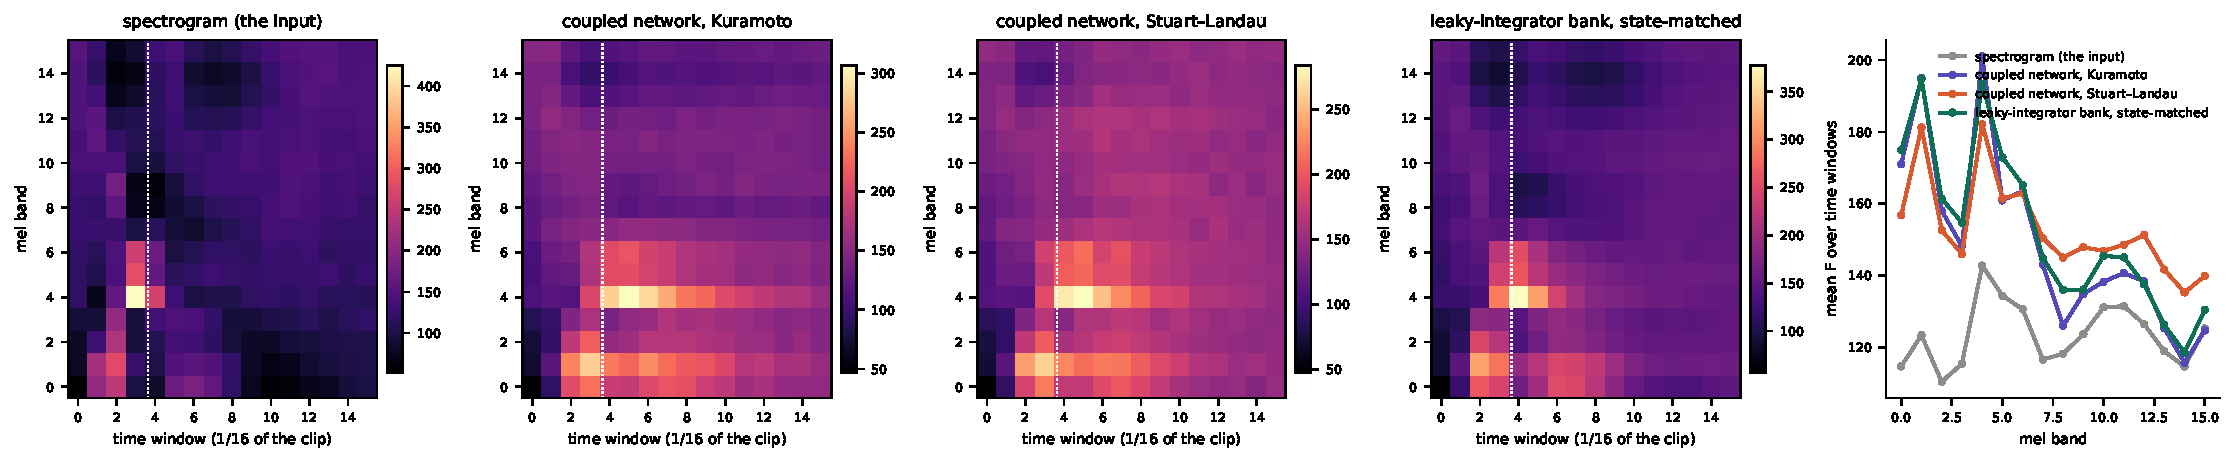
\includegraphics[keepaspectratio,alt={Where each arm carries class information, by one-way ANOVA F over the 2,048 training clips of seed 0 (0 dB, gain 1). Top: mean F per mel band. Below: F per mel band and sixteenth of the clip, each panel on its own colour scale; the dotted line ends the 16-frame warm-up.}]{resources/figures/c7-anova-f.pdf}}
\caption{Where each arm carries class information, by one-way ANOVA F
over the 2,048 training clips of seed 0 (0 dB, gain 1). Top: mean F per
mel band. Below: F per mel band and sixteenth of the clip, each panel on
its own colour scale; the dotted line ends the 16-frame
warm-up.}\label{fig-c7-anova-f}
\end{figure}

\end{document}
